This section evaluates the performance of the cached profile implementation using two recent benchmark suites. The goal is to provide indicators of the performance influence of using cached profiles and analyze where these performance differences come from.
\section{Setup}
\label{s:perf_setup}
To provide reliable and comparable results, all benchmarks are executed on a single node of the Data Center Observatory provided by ETH \cite{ethdco}.
A node features two 8-Core AMD Opteron 6212 CPUs clocked at 2600 MHz with 128 GB of DDR3 RAM and a solid state disk for storage.
A nodes is running Fedora 19 with Linux kernel 3.14.27 and GCC 4.8.3. All JDK builds are compiled on the nodes itself. We use multiple nodes, each benchmark suite is executed on a dedicated node to prevent any influence of inter-node performance differences.
\\\\
The following benchmark suites are used:
\begin{enumerate}
  \item \textbf{SPECjvm 2008:} Developed by Standard Performance Evaluation Corporation, SPECjvm aims to measure the performance of the Java Runtime Environment \cite{specjvm}.  We use version 2008 and we run a subset of 17 out of a total of 21 benchmarks. Four benchmarks are omitted due to incompatibility with OpenJDK 1.9.0.
  \\
  SPECjvm reports the number of operations per minute (ops/m). This is used to compare the performance and more ops/m equals better performance.
  \item \textbf{Octane 2.0:} A benchmark developed by Google to measure the performance of JavaScript code found in large, real-world applications \cite{octane}. Octane runs on Nashorn, a JavaScript Engine of Hotspot. We use version 2.0, which consists of 17 individual benchmarks, of which 16 are compatible with OpenJDK 1.9.0. 
  \\
  Octane gives each benchmark execution a score reflecting the performance. The higher the score, the better the performance.
\end{enumerate}
The benchmark process was automated using a number of self-written Python scripts. Unless specified otherwise, the graphs in this chapter always show the arithmetic mean of 50 runs and the error bars display the 95\% confidence intervals.

\section{Benchmark performance}
\label{s:perf_benchmark}
The main goal of cached profiles is to improve the warmup performance of the JVM. Having a rich profile from an earlier execution will allow the JIT compiler to use a highly optimized version early in method execution.
\\\\
The different profile caching modes were implemented to be able to compare the performance influence of design decisions. We expect the modes to produce different results and the following list suggests reasons for these performance differences:
\begin{itemize}
  \item If the cached profiles fit well in the current method execution, compiling methods with cached profiles earlier than in the baseline will save executions at lower tiers and decrease the time needed for warmup. Benchmarks with these properties should achieve a performance improvement and favor \texttt{Mode 0}.
  \item In case many methods are compiled early, the compile queue could be overloaded and delay compilation of these methods. Also, if a cached profile does not fit the current method execution (the limit of 10 deoptimization was reached, see Section \ref{s:problems}) the JVM will use freshly generated profiles instead. These profiles could be sparse when using lowered compilation thresholds. In these scenarios we expect \texttt{Mode 1} to outperform \texttt{Mode 0}.
  \item \texttt{Mode 2} keeps the steps of the original tiered compilation and is considered the most conservative mode. Also, \texttt{Mode 2} does not modify the compilation thresholds and therefore puts the same load on the compile queue than the baseline version. When using this mode, we can not experience a performance change from earlier compilation but the performance only originates from faster C1 code and the better code quality in C2 due to the cached profiles.
\end{itemize}
\subsection{SPECjvm warmup performance}
\label{s:perf_specjvm_warmup}
The longer a program is running, the less impact a faster warmup has. 
Instead of using SPECjvm's default values, we limited SPECjvm to a single operation, which depending on the benchmark, takes around 6 to 40 seconds.
Additionally, the JVM gets restarted between each single benchmark, to allow an individual analysis and provide full warmup scenarios.
\\\\
We run each benchmark with all cached profiling features disabled. This run is called the \textit{baseline} and displays the original OpenJDK 1.9.0 performance.    
\\\\ 
We then use a single benchmark run, where we configure the JVM to dump the profiling information to disk. By default the benchmark is limited by time and runs for about 6 minutes, including 2 minutes warmup, which do not count towards the performance measurement. The dump profile run is not limited to a single operation but uses the default values of the benchmark instead. The reason is that we want to speed up the warmup. but still keep the same performance for the rest of the benchmark execution. Dumped profiles from a single operation might contain less mature information, which are fine if the benchmark is short running, but could negatively affect long term performance.
\\\\
The profiles gathered are then used in three individual runs by specifying the \texttt{-XX:CacheProfiles} flag. Each run uses one of the three different CacheProfilesModes and the process is repeated 50 times.
%, while the profiles are only recreated after 10 iterations each. This is used to check whether different profile creation runs have any impact on the following performance measurements. However, the evaluation shows that this is not the case.
\begin{figure}[ht!]
  \begin{center}
    \centering
    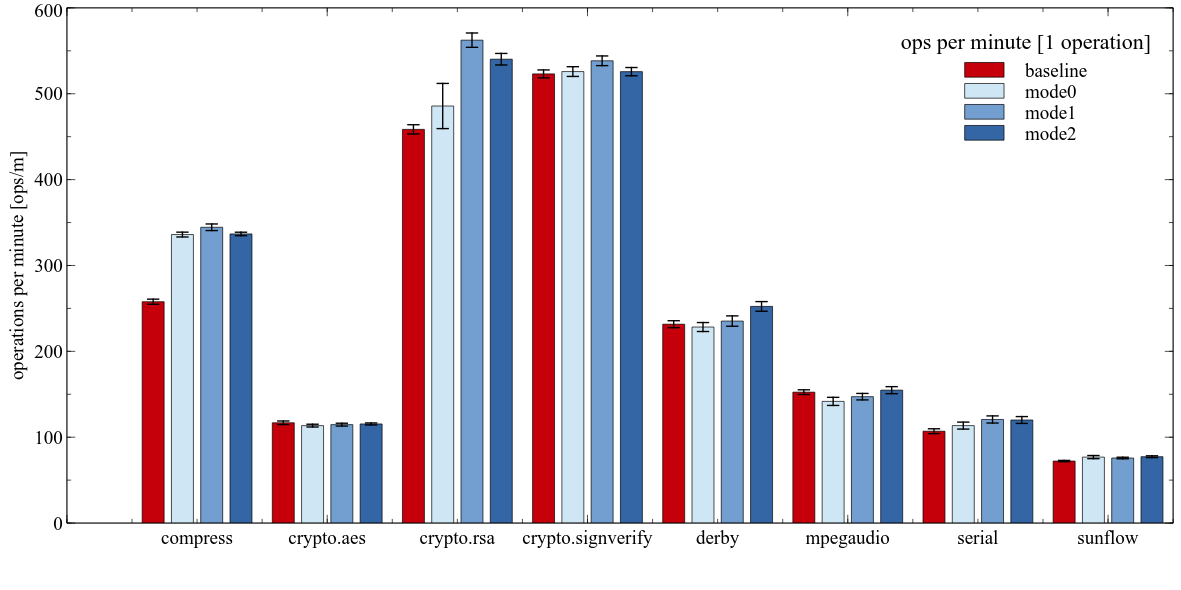
\includegraphics[width=1.0\textwidth]{figures/others_warmup.png}
    \caption{Warmup performance on all different modes (SPECjvm)}
    \label{f:others_warmup}
  \end{center}
\end{figure}
\begin{figure}[ht!]
  \begin{center}
    \centering
    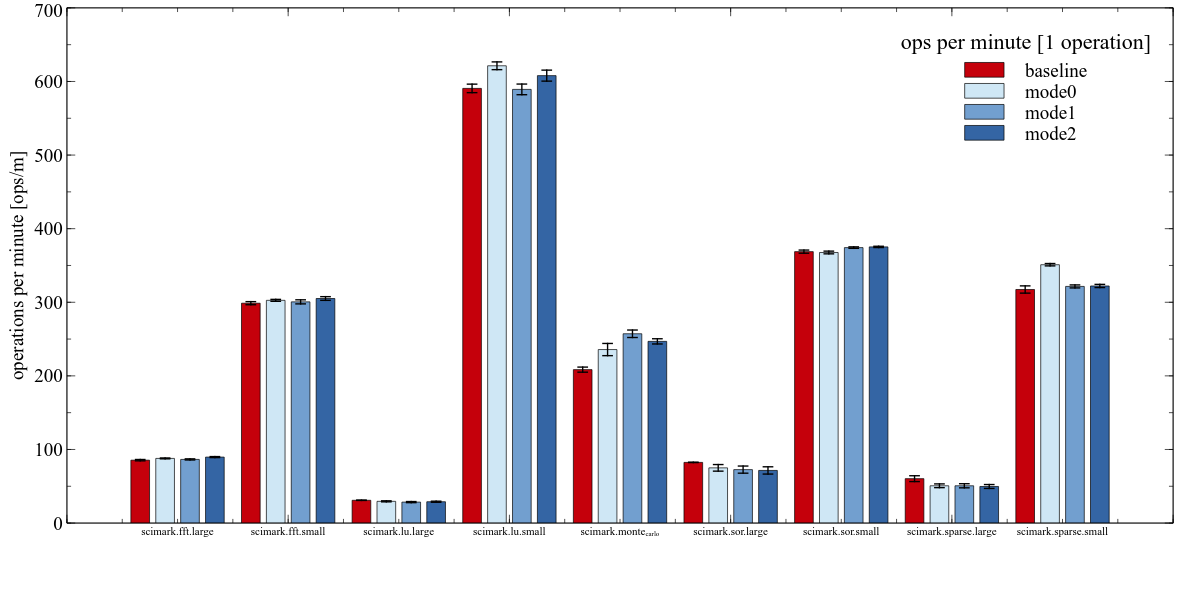
\includegraphics[width=1.0\textwidth]{figures/scimark_warmup.png}
    \caption{Warmup performance on all different modes (SPECjvm scimark)}
    \label{f:scimark_warmup}
  \end{center}
\end{figure}

\begin{figure}[ht!]
  \begin{center}
    \centering
    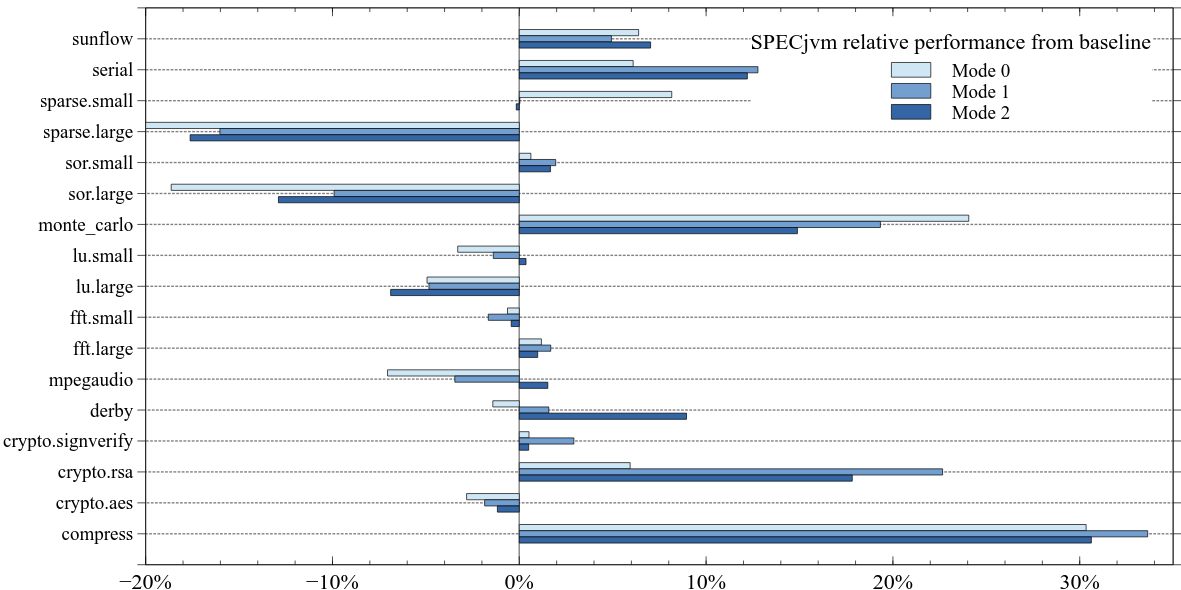
\includegraphics[width=1.0\textwidth]{figures/all_warmup_variation.png}
    \caption{Warmup performance relative to baseline (SPECjvm)}
    \label{f:all_warmup_variation}
  \end{center}
\end{figure}
Figures \ref{f:others_warmup} and \ref{f:scimark_warmup} show the number of operations per minute measured for each benchmark individually. Note, that the operations per minute is not to be confused with the previously mentioned limit of \textit{1 operation} of the benchmark itself.
Figure \ref{f:all_warmup_variation} summarizes the results by showing the relative performance compared to the baseline.
Note, that we omit the "scimark." suffix of the SPECjvm scimark benchmarks for better readability.
\\\\
The individual benchmarks show different effects on performance. We see a performance increase up to around 34\% in the compress benchmark (Mode 1) and a performance decrease of down to 20\% in scimark.sparse.large (Mode 0).
\\\\
Interestingly, the performance differences between the modes are not the same when comparing the individual benchmarks. For example, in crypto.rsa, \texttt{Mode 0} clearly performs worst but in scimark.sparse.small it performs best.
JVM performance is known to be hard to predict and understand \cite{georges2007statistically}. It seems not to be different when cached profiles are used. On average the performance of the benchmark warmup is improved by 2.6\%, 3.4\%, and 2.7\% for Mode 0, Mode 1 and Mode 2.
\\\\
Between the three different modes there is no clear winner. Each mode wins and loses in certain benchmarks against the others in terms of performance. However, in 12 out of 17 benchmarks at least one of the CacheProfileModes improves performance. 
\\\\
As stated before, we expect the influence of cached profiles to be low, when running SPECjvm for the standard duration. Figure \ref{f:all_full_variation} shows the relative performance for all SPECjvm benchmarks running the default duration of 6 minutes.
We see that for most benchmarks, the influence is not significant. That means, using the cached profiles neither increases nor decreases the performance of the long running benchmarks.
However, in sunflow and derby, the performance is worse, especially in \texttt{Mode 0} and \texttt{Mode 1}. Both benchmarks achieve better performance than the baseline when only looking at the warmup. We assume, that in these two cases the cached profiles actually help improving the warmup performance but the code compiled based on these profiles does not contain the same optimizations than the baseline.
\begin{figure}[ht]
  \begin{center}
    \centering
    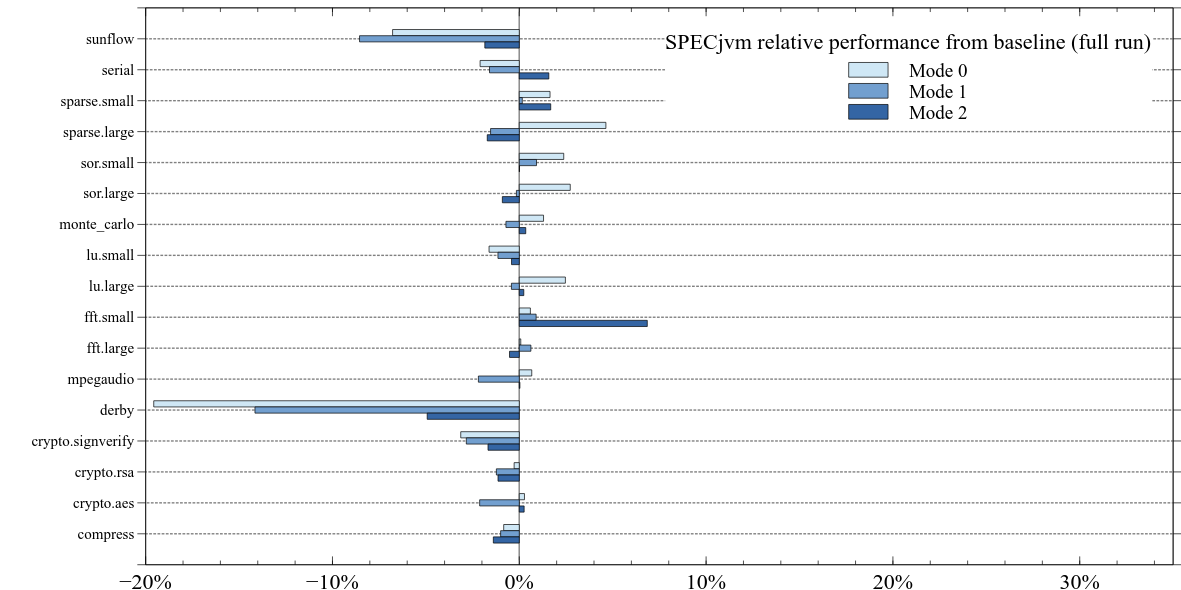
\includegraphics[width=1.0\textwidth]{figures/all_full_variation.png}
    \caption{Performance of a full run relative to baseline (SPECjvm)}
    \label{f:all_full_variation}
  \end{center}
\end{figure} 
\subsection{Octane performance}
\label{s:perf_octane}
Since the individual Octane benchmarks are rather short-running (most of them run for between 4 and 30 seconds) and there is no simple way to run a fixed number of iterations, we run the Octane benchmarks completely. We show performance readings for individual benchmarks. The rest of the setup is identical to SPECjvm in Section \ref{s:perf_specjvm_warmup}.
\\\\
The Octane scores are shown in Figure \ref{f:octane} and a relative comparison with the baseline in Figure \ref{f:octane_variation}.
Compared to SPECjvm the Octane performance is more scattered. The Richards benchmark increases by around 50\% in Mode 0 while NavierStokes decreases by around 25\% in Mode 1. In most benchmarks (9 out of 14) Mode 0 performs worst.
\texttt{Mode 1} and \texttt{Mode 2} generally perform a little bit better, but in total only 6 out of 14 benchmarks result in a performance improvement in at least one mode.
On average the performance differences over all individual benchmarks compared to the baseline are -5.9\%, 0.6\%, and 0.1\% for Mode 0, Mode 1 and Mode 2.
\begin{figure}[ht]
  \begin{center}
    \centering
    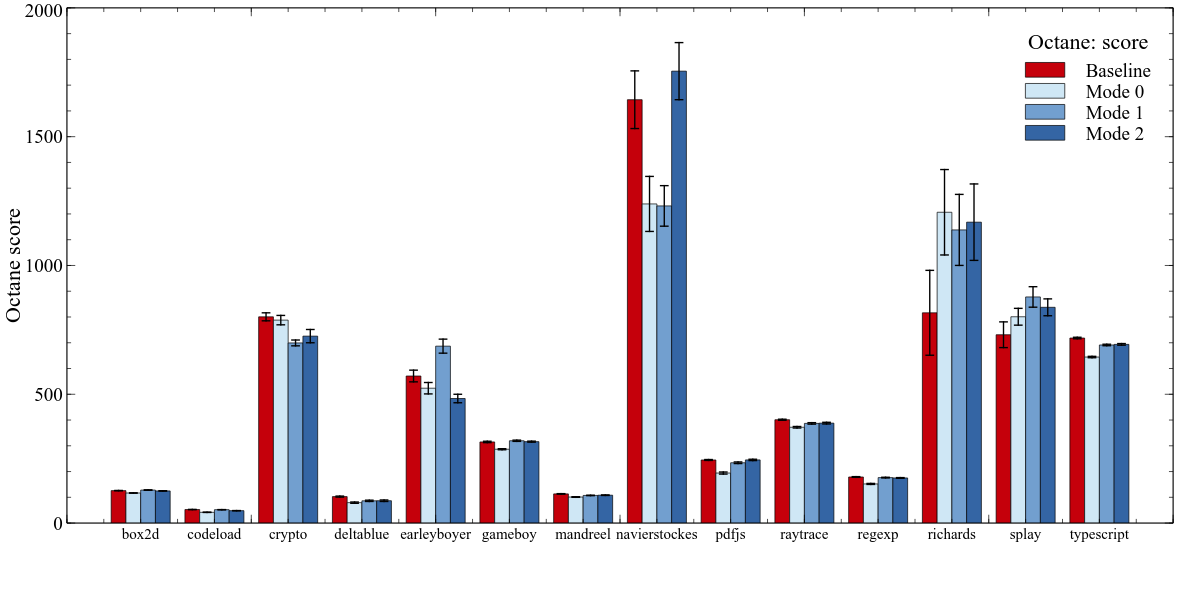
\includegraphics[width=1.0\textwidth]{figures/octane.png}
    \caption{performance on all different modes (Octane)}
    \label{f:octane}
  \end{center}
\end{figure}

\begin{figure}[ht]
  \begin{center}
    \centering
    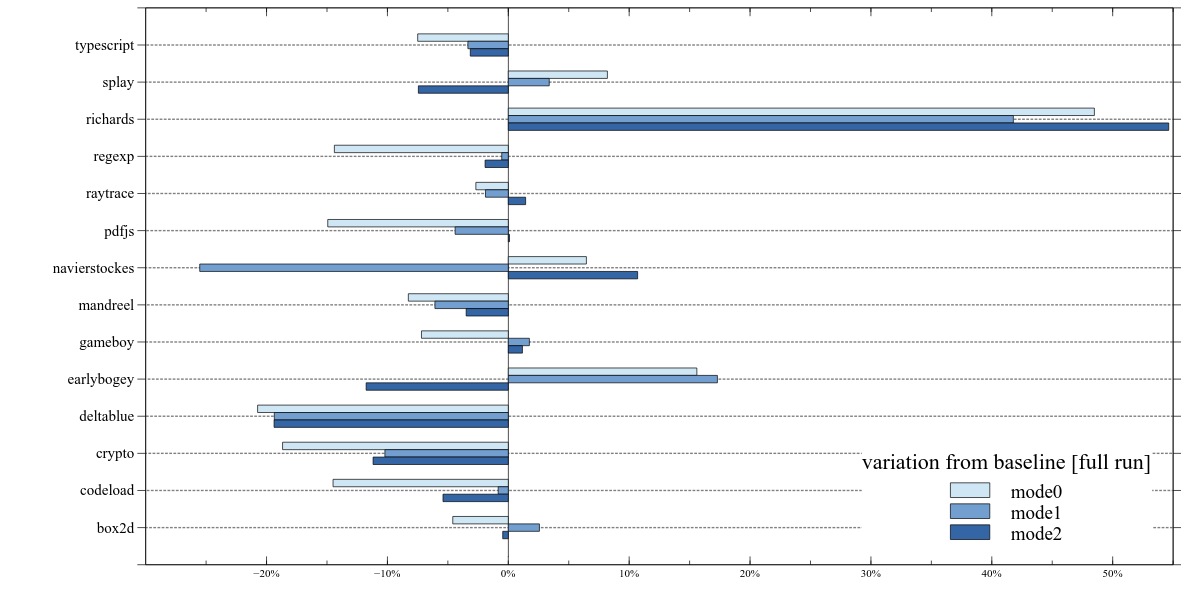
\includegraphics[width=1.0\textwidth]{figures/octane_variation.png}
    \caption{Performance relative to baseline (Octane)}
    \label{f:octane_variation}
  \end{center}
\end{figure}
\clearpage
\section{Deoptimizations}
\label{s:perf_deoptimizations}
We aim to lower the time needed for warmup by compiling methods earlier and at lower tiers. We also expect to decrease the number of deoptimizations by having more complete profiles available earlier, which ideally results in better compiled code quality. To measure the total amount of deoptimizations we implemented a new compiler flag \texttt{-XX:+PrintDeoptimizationCount}.
The number of deoptimizations of the SPECjvm benchmarks are shown in Figure \ref{f:others_warmup_deopt} and Figure \ref{f:scimark_warmup_deopt}. The Octane numbers are drawn in Figure \ref{f:octane_deopt}.
Again, we also included graphs that show the number of deoptimizations relative to the baseline runs in Figure \ref{f:all_warmup_variation_deopt} and Figure \ref{f:octane_variation_deopt}.
\\\\
The measurements show that when using \texttt{Mode 1} or \texttt{Mode 2}, we are able to reduce the deoptimizations significantly in all benchmarks except one (GameBoy). In \texttt{Mode 0}, there is a clear difference between SPECjvm and Octane. While in SPECjvm the number of deoptimizations is similar to the other modes, in Octane \texttt{Mode 0} increases the number by 30\%. \texttt{Mode 0} also has the largest performance regression in Octane, the high amount of deoptimizations could be a sign for this result. 
\\\\
And, while a low deoptimization number is a good indication of the increased code quality for methods being compiled with cached profiles, we could not find a direct correlation between number of deoptimizations and the performance results.
\\\\
One possible reason is that the amount of deoptimizations does not necessarily describe the performance impact. Especially, when considering multi-threaded systems, there can be a large number of deoptimizations in performance uncritical threads that are avoided by using cached profiles and therefore heavily reduce the total counter. But if there is one very important method in a performance critical thread, which has executions that are not reflected in the cached profiles, this method could trigger only very few deoptimizations but still influence performance significantly.
\begin{figure}[ht]
  \begin{center}
    \centering
    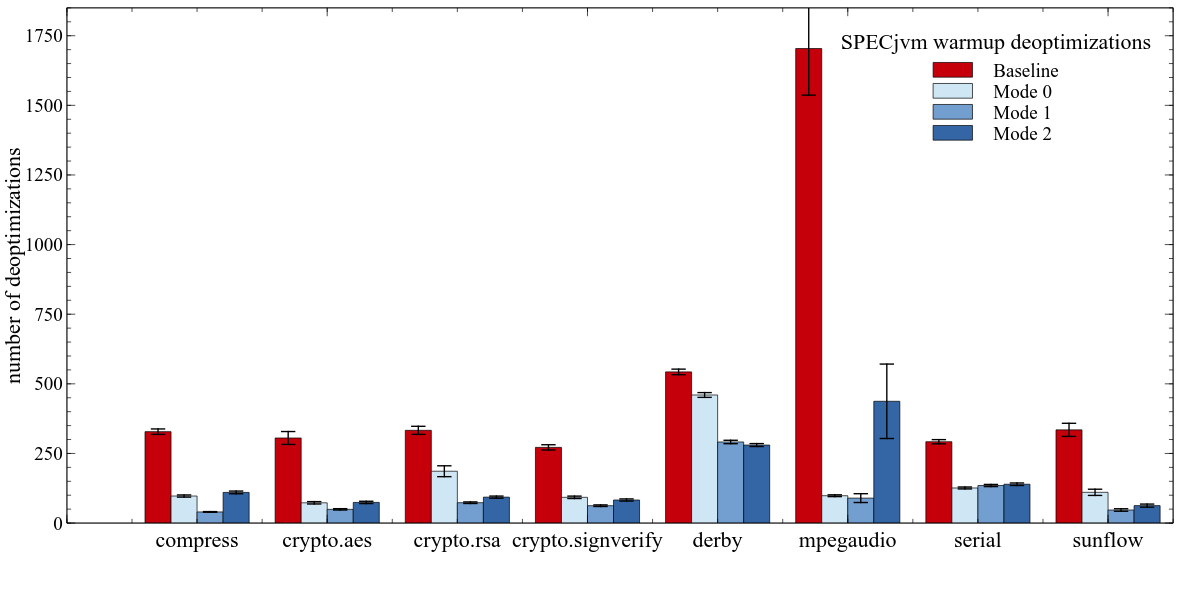
\includegraphics[width=1.0\textwidth]{figures/others_warmup_deopt.png}
    \caption{Deoptimizations of all modes (SPECjvm)}
    \label{f:others_warmup_deopt}
  \end{center}
\end{figure}
\begin{figure}[ht]
  \begin{center}
    \centering
    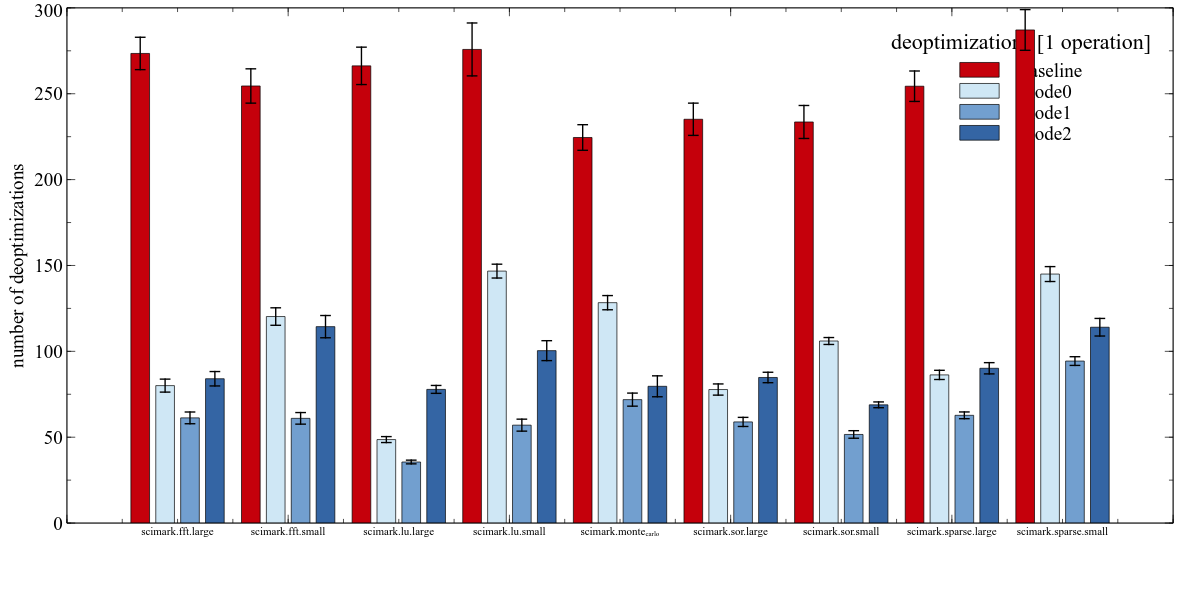
\includegraphics[width=1.0\textwidth]{figures/scimark_warmup_deopt.png}
    \caption{Deoptimizations of all modes (SPECjvm scimark)}
    \label{f:scimark_warmup_deopt}
  \end{center}
\end{figure}
\begin{figure}[ht]
  \begin{center}
    \centering
    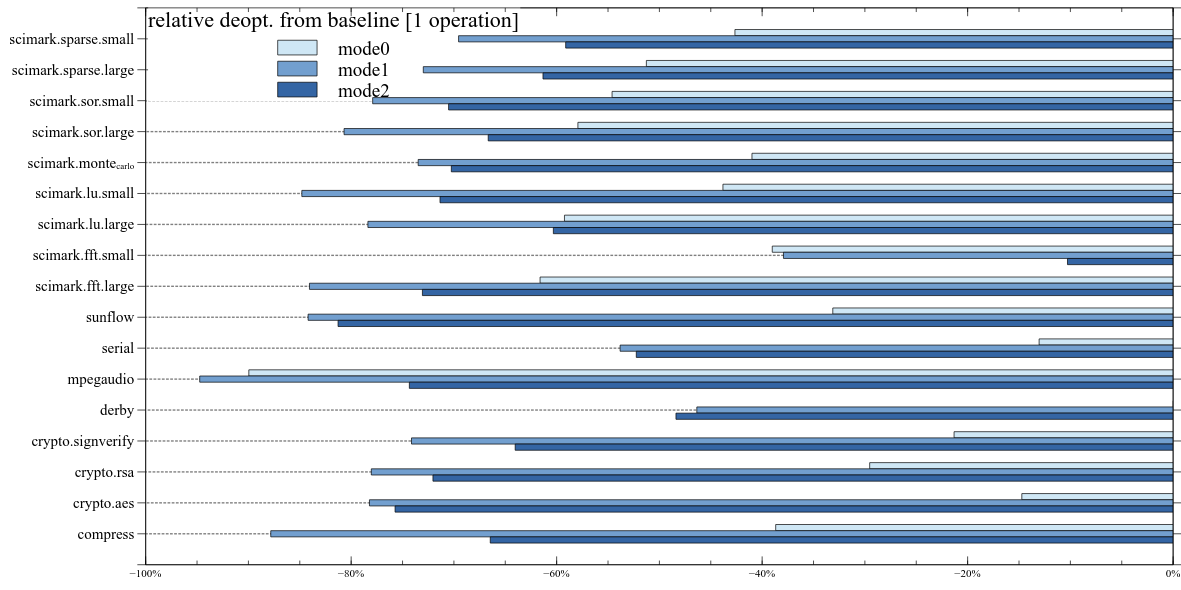
\includegraphics[width=1.0\textwidth]{figures/all_warmup_variation_deopt.png}
    \caption{Change in the number of deoptimizations relative to baseline (SPECjvm)}
    \label{f:all_warmup_variation_deopt}
  \end{center}
\end{figure}
\begin{figure}[ht]
  \begin{center}
    \centering
    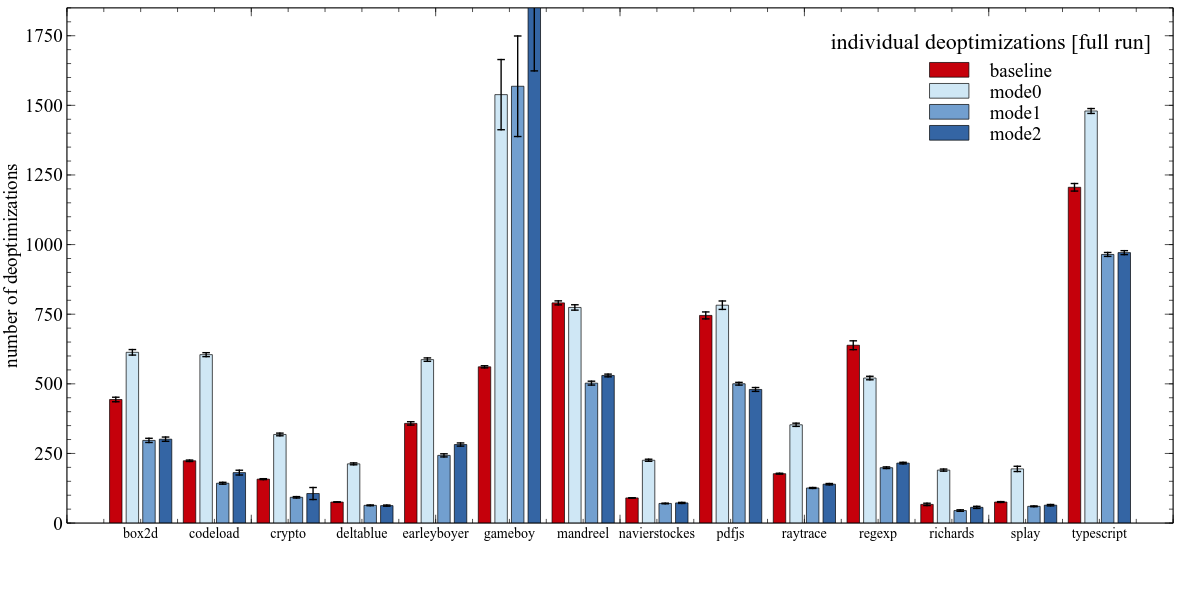
\includegraphics[width=1.0\textwidth]{figures/octane_deopt.png}
    \caption{Deoptimizations of all modes (Octane)} 
    \label{f:octane_deopt}
  \end{center}
\end{figure}
\begin{figure}[ht]
  \begin{center}
    \centering
    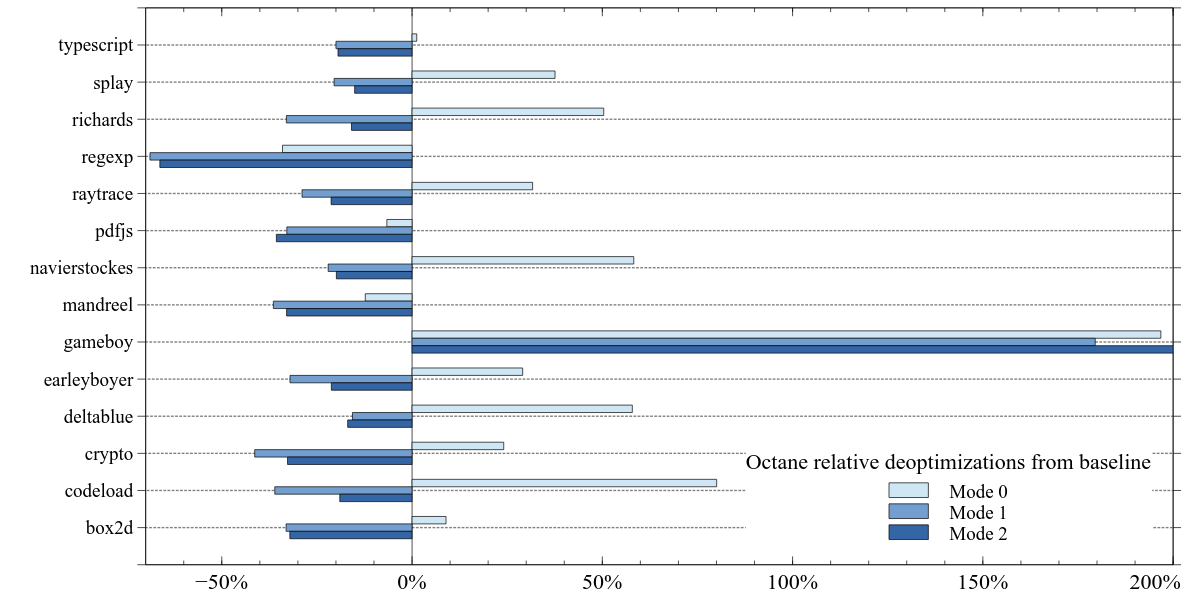
\includegraphics[width=1.0\textwidth]{figures/octane_variation_deopt.png}
    \caption{Change in the number of deoptimizations relative to baseline (Octane)}
    \label{f:octane_variation_deopt}
  \end{center}
\end{figure}
\clearpage
\section{Effect on compile queue}
\label{s:perf_compilequeue}
When designing the different CacheProfilesModes we thought, that lowering the compilation thresholds will increase the load on the compiler, especially early in program execution. This results in the compiler not being able to handle all requests immediately and the compile queue fills up. Execution of compiled methods can be delayed and therefore performance degradation occur.
\\\\
We added a new HotSpot flag \texttt{-XX:+PrintCompileQueueSize}, which allows us to trace the current number of methods that are scheduled for compilation. We selected 6 individual benchmarks and printed their C1 and C2 compile queue for all three CacheProfileModes in Figure \ref{f:octane_queue_richards_separate_c1} to Figure \ref{f:octane_queue_deltablue_separate_c2}.
The selected benchmarks and the reason why an individual analysis was performed are listed below:
\begin{itemize}
  \item \textbf{Octane Richards:} This benchmarks achieved the highest performance benefit from using cached profiles in all three modes. We are interested to see if the compile queue load differs from worse performing benchmarks.
  \item \textbf{Octane EarleyBoyer:} This is a benchmark, where \texttt{Mode 1} performs significantly better than the other two modes. We chose this to benchmark, whether \texttt{Mode 1} shows a different compile queue behavior.
  \item \textbf{Octane NavierStokes:} Navierstokes has a 8\% performance increase in \texttt{Mode 2} but a 25\% performance decrease in \texttt{Mode 0} and \texttt{Mode 1}. Motivation is the same as EarleyBoyer, except we focus on \texttt{Mode 2}.
  \item \textbf{Octane Deltablue:} This benchmark achieves the highest performance loss from using cached profiles in all three modes. Together with the best performing benchmark (Richards) we are interested, if the load on the compile queue indicates any performances differences.
  \item \textbf{SPECjvm compress:} Compress is the best performing SPECjvm benchmark when using cached profiles. 
  \item \textbf{SPECjvm scimark.sparse.large:} This is the worst performing SPECjvm benchmark when using cached profiles. 
\end{itemize}
The reason for the runs using cached profiles starting their main amount of compilations later than the baseline, is because the JVM must parse the cached profile file first.
\\\\
We realize that analyzing the compile queue does not really help us understanding the performance variations when cached profiles are used.
The graphs that show the C1 compile queue size over time, do not significantly differ from the baseline, nor is there a difference between the individual modes.
\\\\
For C2, we can not correlate the variation of the compile queue size over time with the benchmark performance.
\\\\
Figure \ref{f:octane_queue_richards_separate_c2} shows the C2 compile queue of the Octane Richards benchmark. As expected, due to removing steps from the tiered compilation, we increased the load on C2 in \texttt{Mode 0} and \texttt{Mode 1} with compile queue peaks at around 20 scheduled compilations. Nevertheless, these modes have a performance increase of close to 50\% better than the baseline. \texttt{Mode 2}, which was designed to keep the original tiered compilation steps unmodified, does not have similar peaks but nevertheless achieves similar performance.
\\\\
EarleyBoyer's compile queue is displayed in Figure \ref{f:octane_queue_richards_separate_c2}. \texttt{Mode 1} performs better than the other two modes and compared to \texttt{Mode 0} puts even more pressure on the compile queue.
It is interesting, that in this particular benchmark, even the baseline version puts a lot of pressure on the compile queue early on.
\\\\
In Figure \ref{f:octane_queue_navierstokes_separate_c2} we see NavierStokes' compile queue. \texttt{Mode 2} performs best but we can not derive any indications why this is the case from looking at the queue size.
\\\\
The Deltablue benchmark shown in Figure \ref{f:octane_queue_deltablue_separate_c2} has the worst performance when using cached profiles but the compile queue size looks very similar to the one of the Richards benchmark, where performance is significantly better.
\\\\
We will abstain from looking at the SPECjvm benchmarks, since they do not offer any new insights. The graphs can be found in the Appendix \ref{a:additional_graphs}.
\\\\
The detailed analysis of the compile queue shows, that our thoughts about the effect on the compile queue were not unfounded for most of the selected benchmarks. However, we were not able to relate these influences to actual performance effects. Especially, overloading the compile queue does not necessarily affect performance negatively.
% --------------------------- Octane Richards Queue ------------------
\begin{figure}[ht]
  \begin{center}
    \centering
    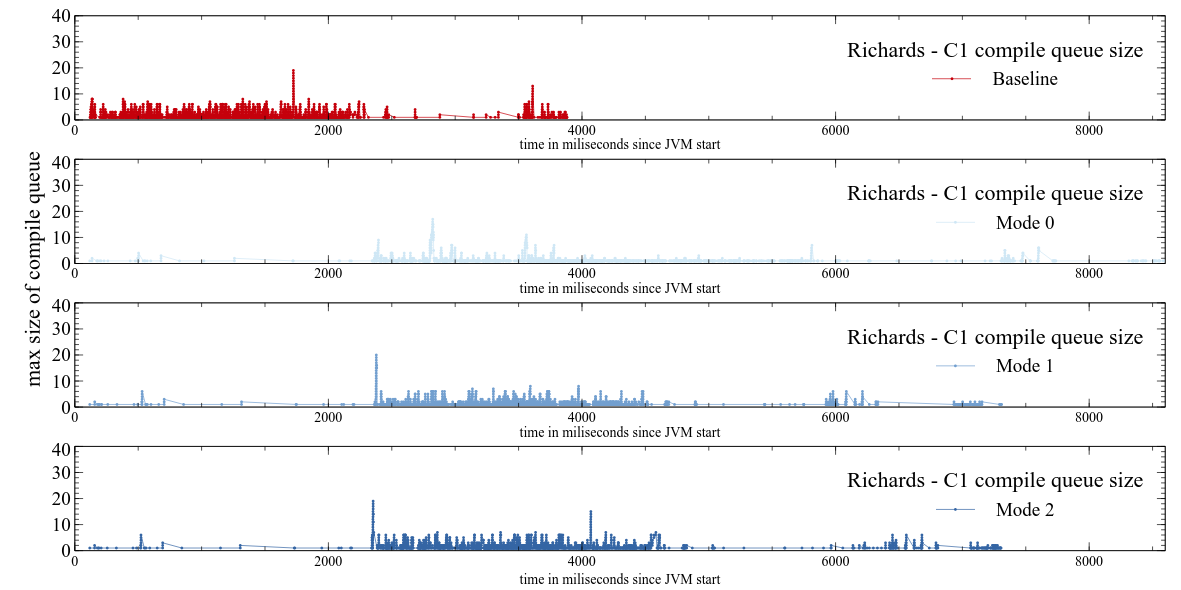
\includegraphics[width=1.0\textwidth]{figures/octane_queue_richards_separate_c1.png}
    \caption{C1 Compile queue size over time Octane Richards benchmark}
    \label{f:octane_queue_richards_separate_c1}
  \end{center}
\end{figure}
\begin{figure}[ht]
  \begin{center}
    \centering
    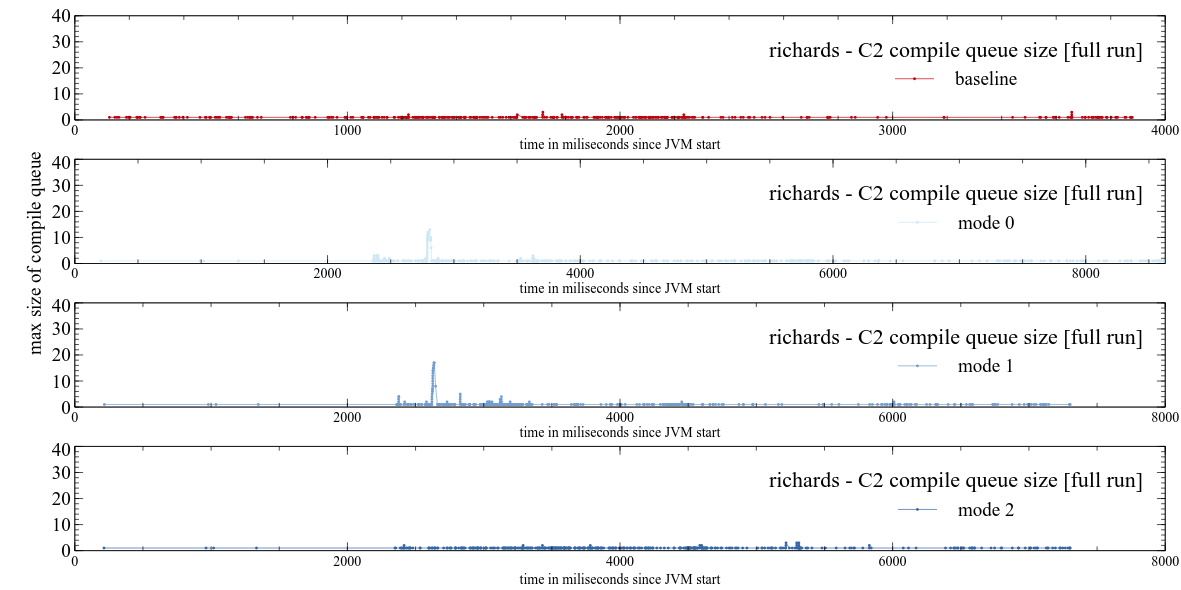
\includegraphics[width=1.0\textwidth]{figures/octane_queue_richards_separate_c2.png}
    \caption{C2 Compile queue size over time Octane Richards benchmark}
    \label{f:octane_queue_richards_separate_c2}
  \end{center}
\end{figure}
% --------------------------- Octane EarleyBoyer Queue ------------------
\begin{figure}[ht]
  \begin{center}
    \centering
    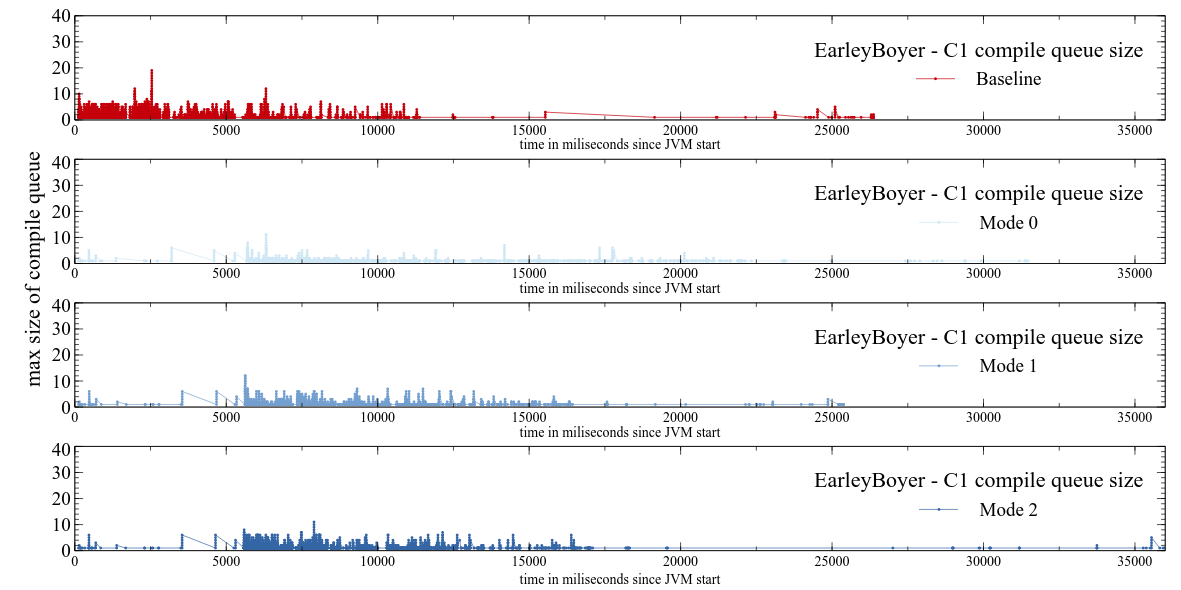
\includegraphics[width=1.0\textwidth]{figures/octane_queue_earleyboyer_separate_c1.png}
    \caption{C1 Compile queue size over time Octane EarleyBoyer benchmark}
    \label{f:octane_queue_earleyboyer_separate_c1}
  \end{center}
\end{figure}
\begin{figure}[ht]
  \begin{center}
    \centering
    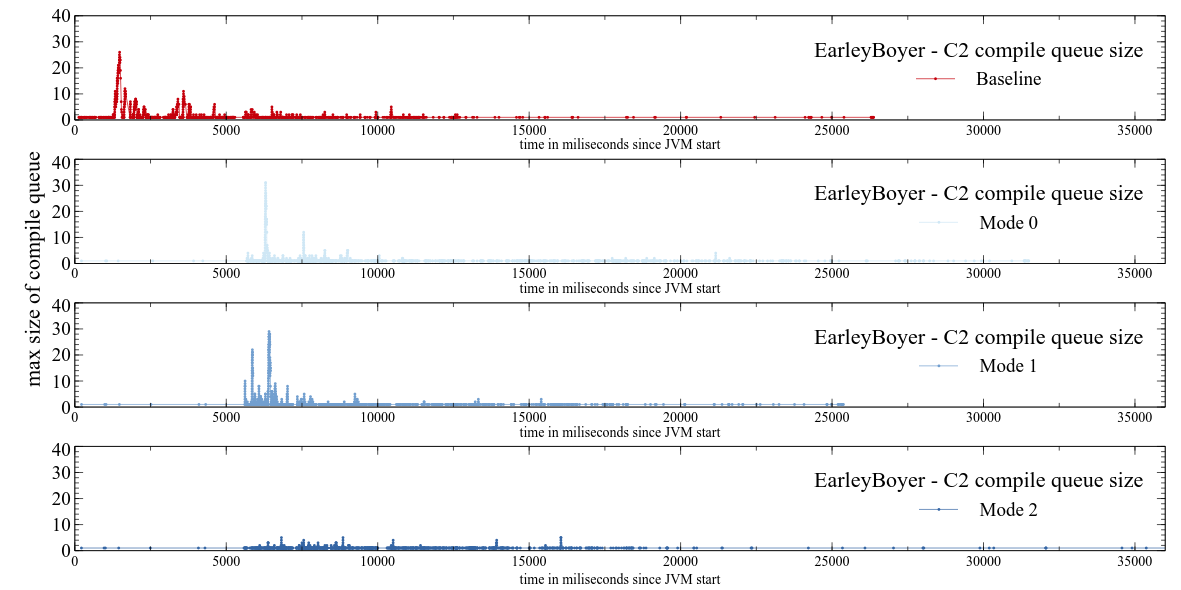
\includegraphics[width=1.0\textwidth]{figures/octane_queue_earleyboyer_separate_c2.png}
    \caption{C2 Compile queue size over time Octane EarleyBoyer benchmark}
    \label{f:octane_queue_earleyboyer_separate_c2}
  \end{center}
\end{figure}
% --------------------------- Octane NavierStokes Queue ------------------
\begin{figure}[ht]
  \begin{center}
    \centering
    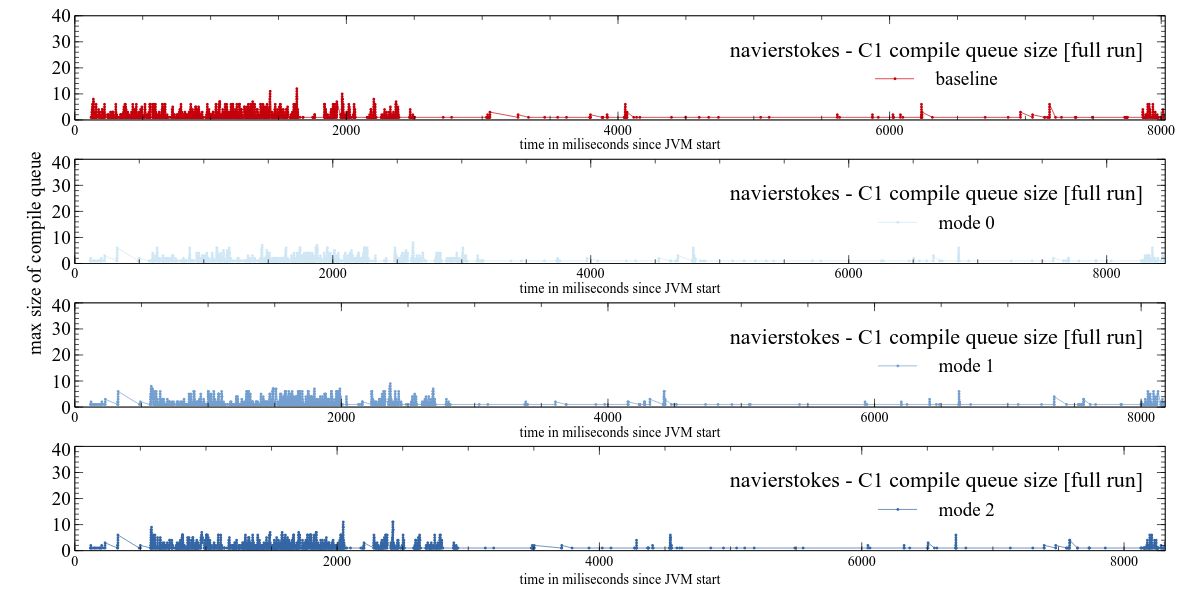
\includegraphics[width=1.0\textwidth]{figures/octane_queue_navierstokes_separate_c1.png}
    \caption{C1 Compile queue size over time Octane NavierStokes benchmark}
    \label{f:octane_queue_navierstokes_separate_c1}
  \end{center}
\end{figure}
\begin{figure}[ht]
  \begin{center}
    \centering
    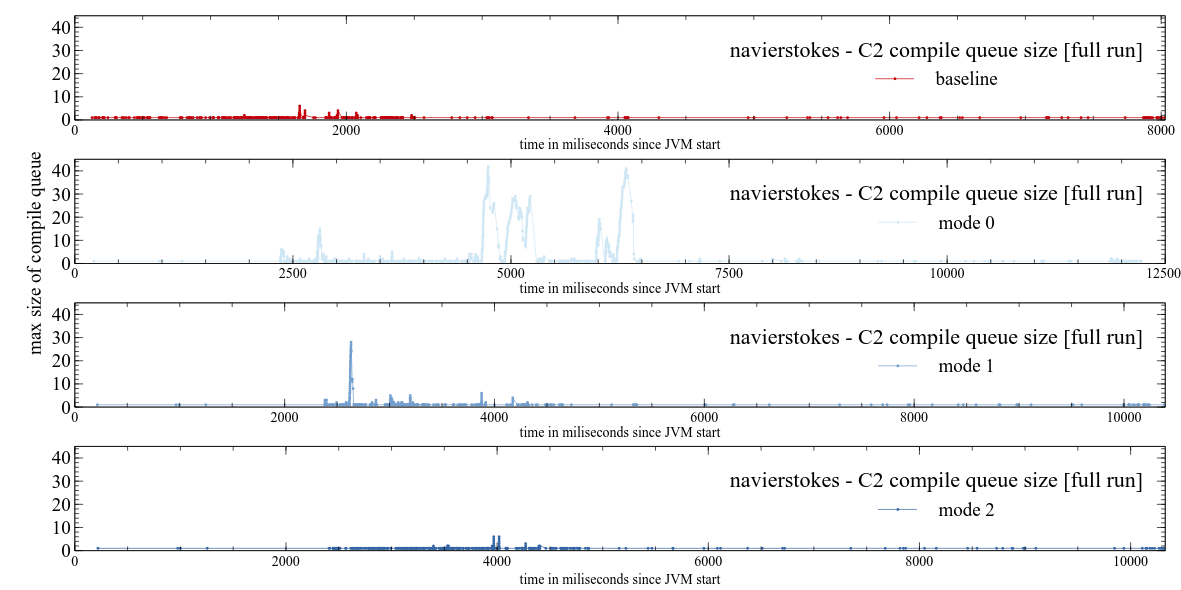
\includegraphics[width=1.0\textwidth]{figures/octane_queue_navierstokes_separate_c2.png}
    \caption{C2 Compile queue size over time Octane NavierStokes benchmark}
    \label{f:octane_queue_navierstokes_separate_c2}
  \end{center}
\end{figure}
% --------------------------- Octane DeltaBlue Queue ------------------
\begin{figure}[ht]
  \begin{center}
    \centering
    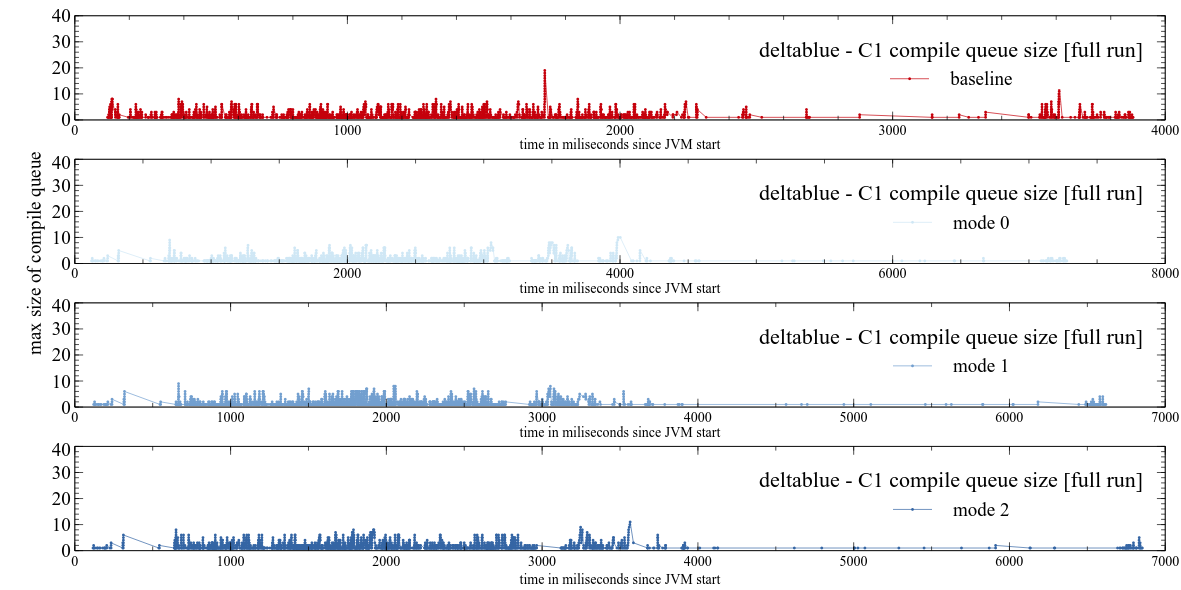
\includegraphics[width=1.0\textwidth]{figures/octane_queue_deltablue_separate_c1.png}
    \caption{C1 Compile queue size over time Octane Deltablue benchmark}
    \label{f:octane_queue_deltablue_separate_c1}
  \end{center}
\end{figure}
\begin{figure}[ht]
  \begin{center}
    \centering
    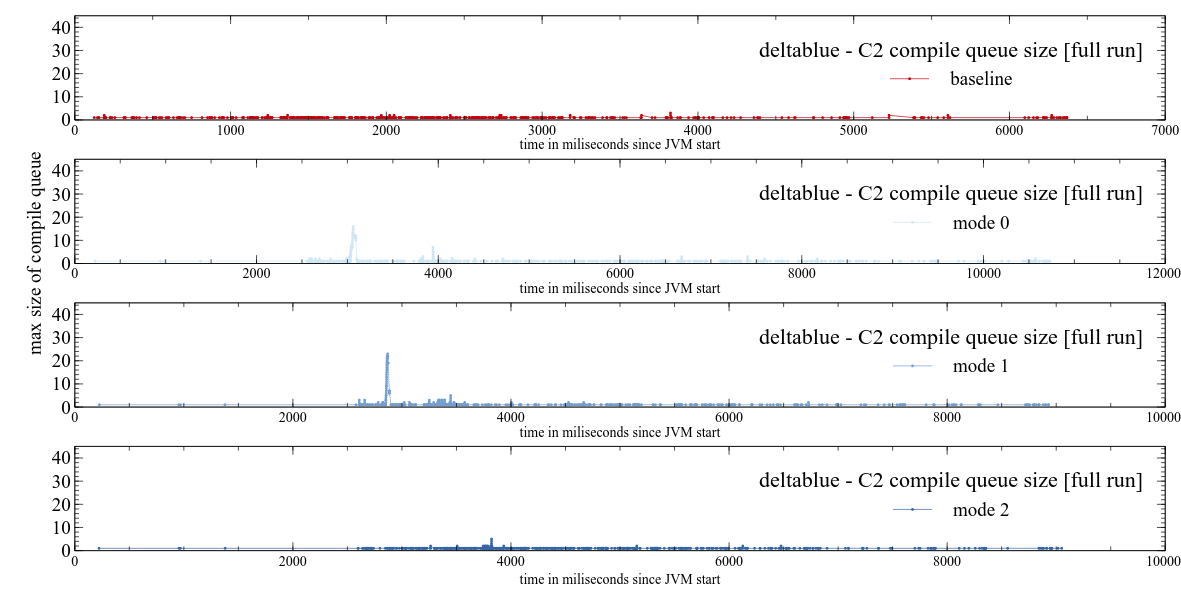
\includegraphics[width=1.0\textwidth]{figures/octane_queue_deltablue_separate_c2.png}
    \caption{C2 Compile queue size over time Octane Deltablue benchmark}
    \label{f:octane_queue_deltablue_separate_c2}
  \end{center}
\end{figure}
\clearpage

\section{Number and type of compilations}
\label{s:perf_compilenumber}
In this section, we take a look on how cached profile modify the ratio of C1 and C2 compilations and if there is a correlation between percentage of methods using cached profiles and the resulting performance.
\\\\
We continue the focus on the 6 individual benchmarks, selected in Section \ref{s:perf_compilequeue}.
We use the newly added HotSpot flag \texttt{-XX:+PrintCacheProfiles}, that prints out the level of each compilation and whether or not it uses cached profiles.
% --------------------------- Queue Total ------------------
\begin{figure}[ht!]
  \begin{center}
    \centering
    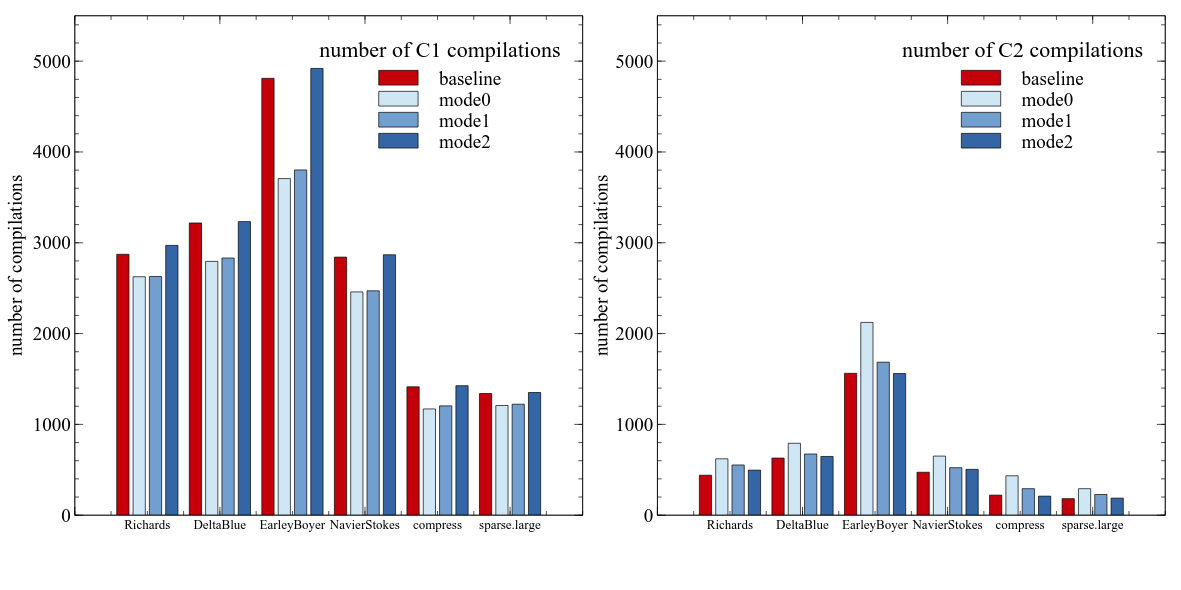
\includegraphics[width=1.0\textwidth]{figures/queue_total.png}
    \caption{Number of compilations for some specJVM and octane benchmarks}
    \label{f:queue_total}
  \end{center}
\end{figure}
\\
Figure \ref{f:queue_total} shows the total amount of compilations, split between C1 and C2.
We see, that the Octane benchmarks and the SPECjvm benchmarks behave differently. While the 4 Octane ones achieve a lower amount of C1 compilations in \texttt{Mode 0} and \texttt{Mode 1}, \texttt{Mode 2} is similar to the baseline. The two SPECjvm benchmarks have more C1 compilations in \texttt{Mode 0}, less in \texttt{Mode 1} and the same amount in \texttt{Mode 2} compared to the baseline.
\\\\
The changes of the amount of C2 compilations are very similar in all benchmarks. Using \texttt{Mode 0} and \texttt{Mode 1} results in more C2 compilations than the baseline and \texttt{Mode 2} achieves around the same amount as the baseline.
\\\\
If we recall the differences between the modes, these results make sense. \texttt{Mode 0} lowers the thresholds of C1 compilations in case the method has a cached profile and compiles with C2 instead. This reduces the number of C1 compilations in favor of more C2 compilations. \texttt{Mode 1} does not lower the thresholds but it still promotes some C1 compilations to C2 compilations due to the fact that C1 requests of methods with a cached profile get compiled with C2 immediately.
\texttt{Mode 2} leaves the tiered compilation completely untouched and therefore has very similar compilation numbers to the baseline.
\\\\
Furthermore, we are interested how many of the compilations use cached profiles. We want to be as close to 100\% as possible, but the experiments show that around 65\%-70\% of the compilations use cached profiles.
The reason is that the compilation replay functionality does not support certain methods, e.g. lambda expressions. For lambda expressions, the JVM generates classes during runtime. Because the class names might differ it is hard to correlate cached profiles to classes of lambda expressions. Since the profile caching implementation is based on compilation replay, it will also not compile these methods using cached profiles. 
Additionally, we do not use any profiles for compilation Level 1 and Level 2 as described in Section \ref{s:usingprofiles}.
\\\\
In Figure \ref{f:richards_compilations} to Figure \ref{f:sparselarge_compilations} we show pie charts, that visualize the portion of specific compilation types.
When comparing different benchmarks of the same CacheProfilesMode, we realize that the share of each compile type is constant.
The pie charts of \texttt{Mode 0} and \texttt{Mode 1} differ only slightly. In all benchmarks, using \texttt{Mode 1} invokes less compilations using cached profiles than \texttt{Mode 1}.
In \texttt{Mode 2}, we see Level 2 compilations appear, due to the changed tiered compilation transitions. The number of Level 3 compilations is almost unchanged compared to \texttt{Mode 1}, because these are compilations of methods where no profiles from C2 compilations are available.
The Level 2 compilations only happen if a C2 profile is cached and usually result in additional Level 4 compilations. 
% --------------------------- Compilation cake Richards ------------------
\begin{figure}[ht]
  \begin{center}
    \centering
    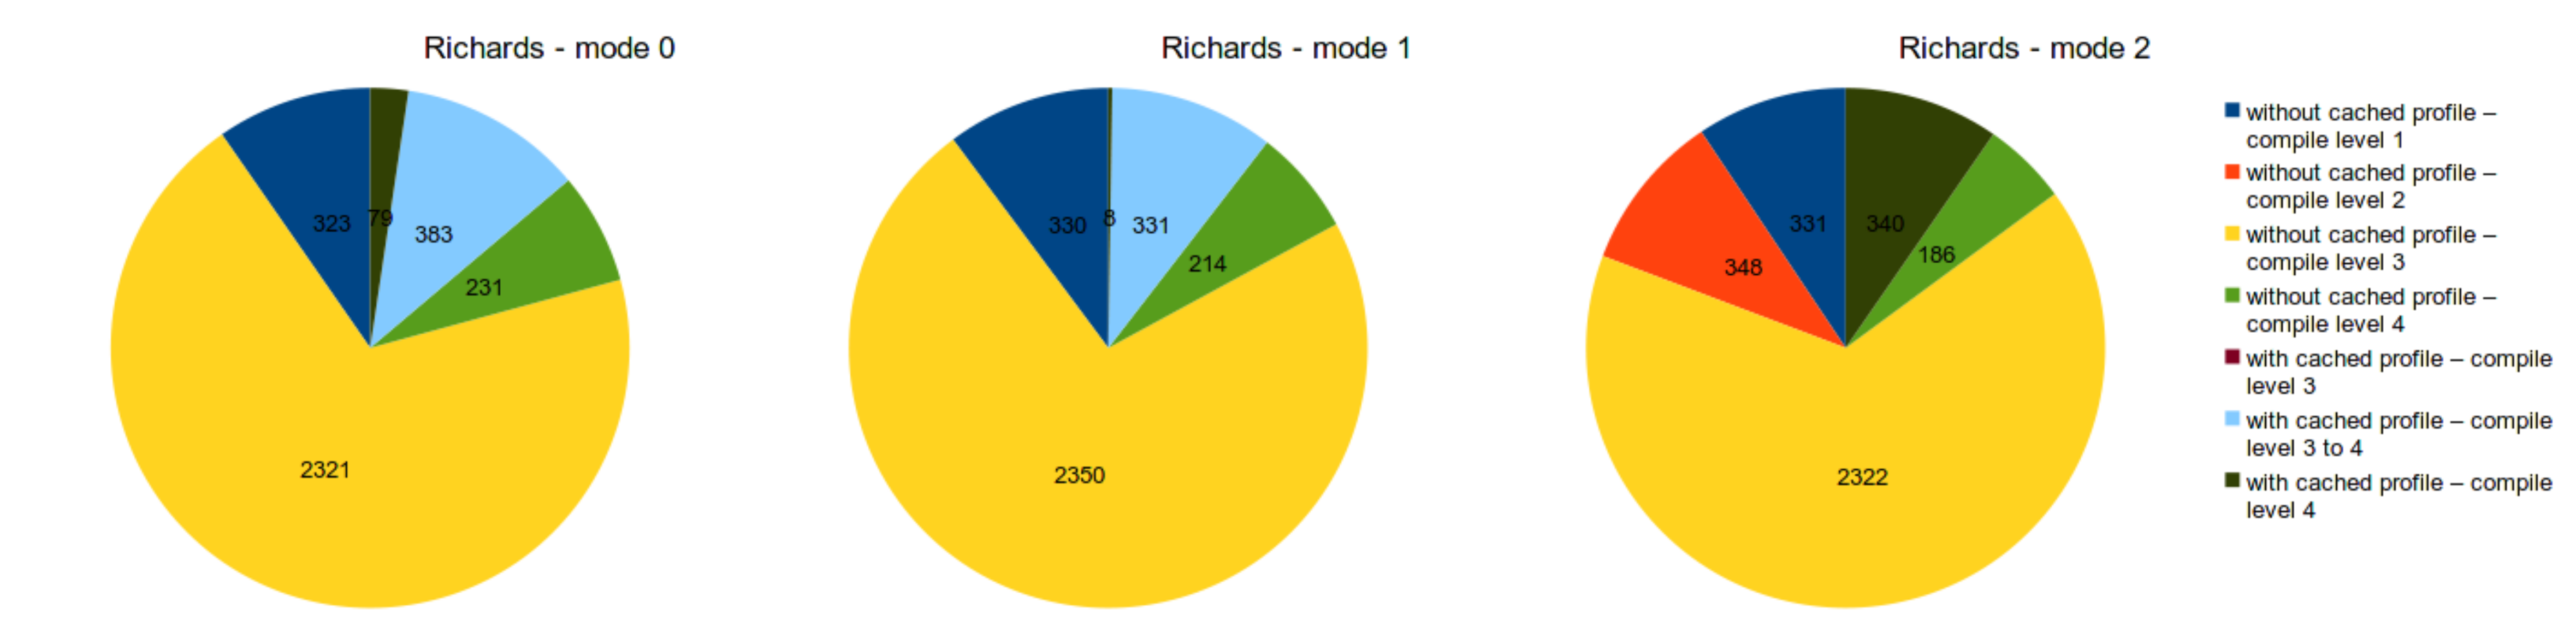
\includegraphics[width=1.0\textwidth]{figures/richards_compilations.png}
    \caption{Ratio of compilations Octane Richards benchmark}
    \label{f:richards_compilations}
  \end{center}
\end{figure}
% --------------------------- Compilation cake Richards ------------------
\begin{figure}[ht]
  \begin{center}
    \centering
    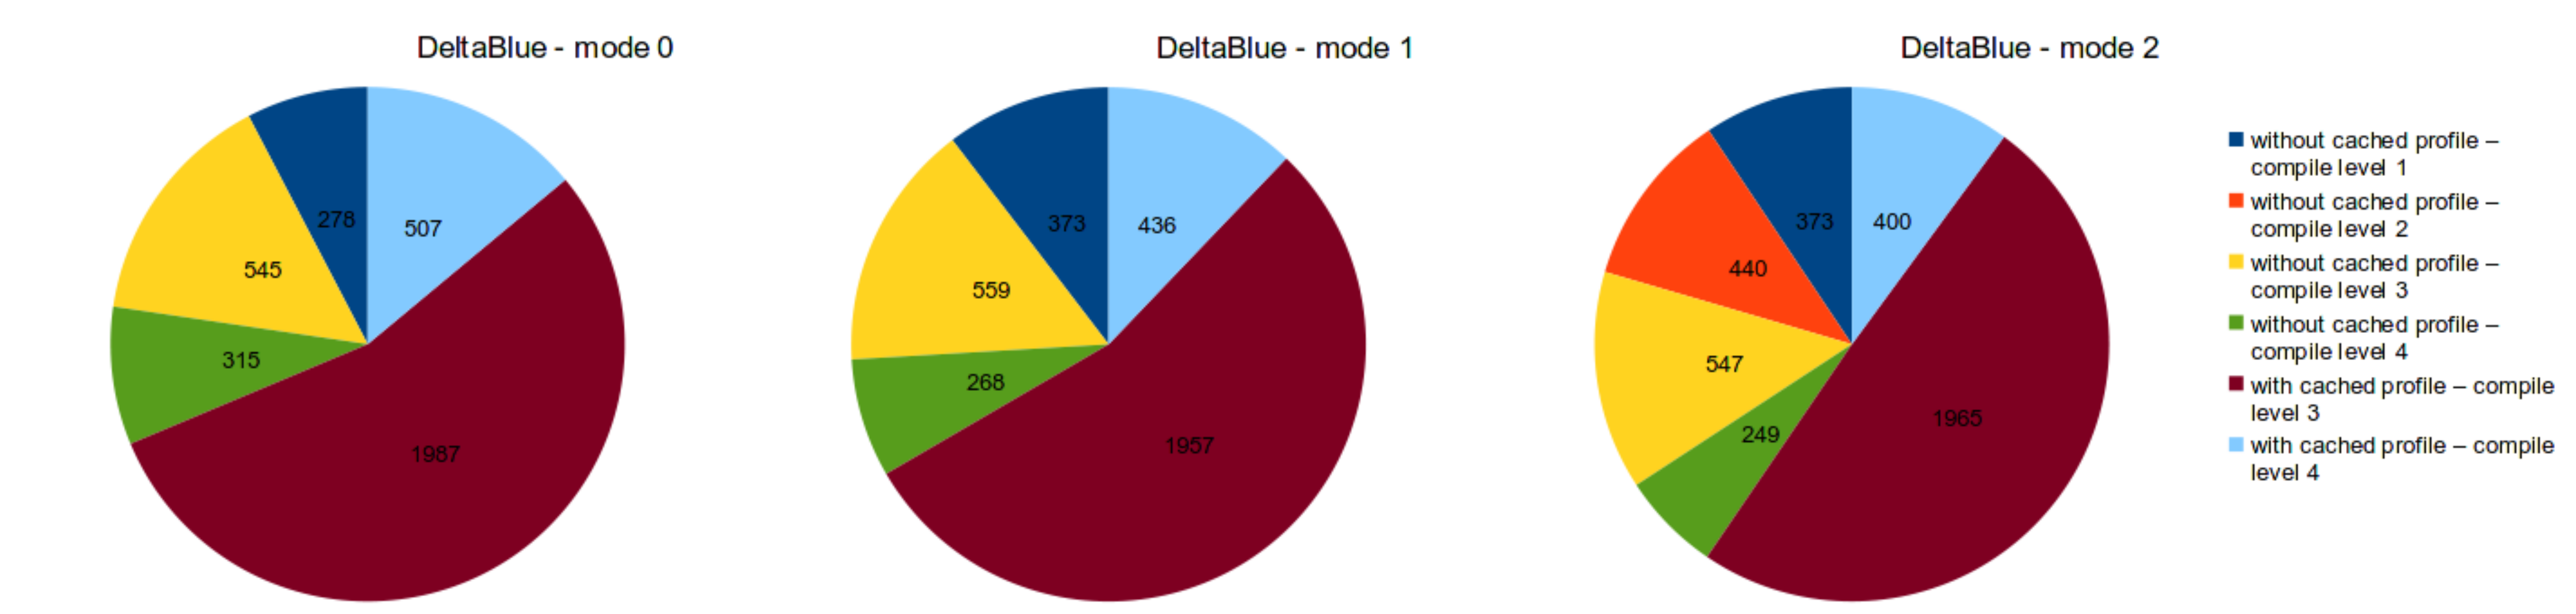
\includegraphics[width=1.0\textwidth]{figures/deltablue_compilations.png}
    \caption{Ratio of compilations Octane Deltablue benchmark}
    \label{f:deltablue_compilations}
  \end{center}
\end{figure}
% --------------------------- Compilation cake Richards ------------------
\begin{figure}[ht]
  \begin{center}
    \centering
    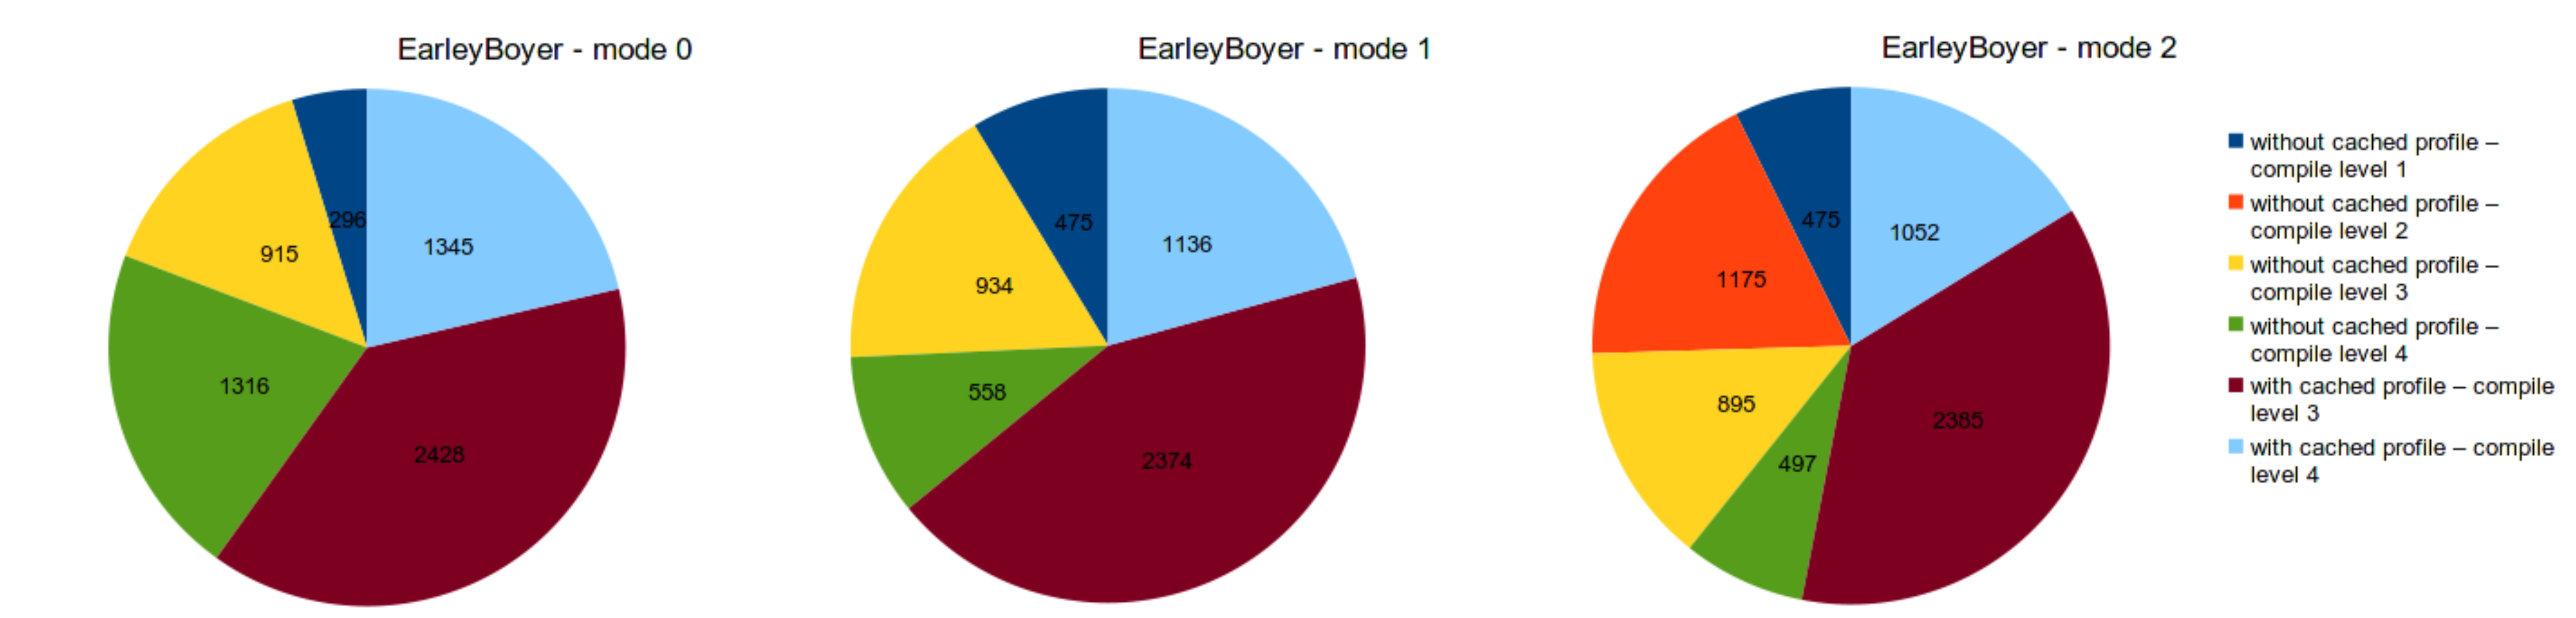
\includegraphics[width=1.0\textwidth]{figures/earleyboyer_compilations.png}
    \caption{Ratio of compilations Octane EarleyBoyer benchmark}
    \label{f:earleyboyer_compilations}
  \end{center}
\end{figure}
% --------------------------- Compilation cake Richards ------------------
\begin{figure}[ht]
  \begin{center}
    \centering
    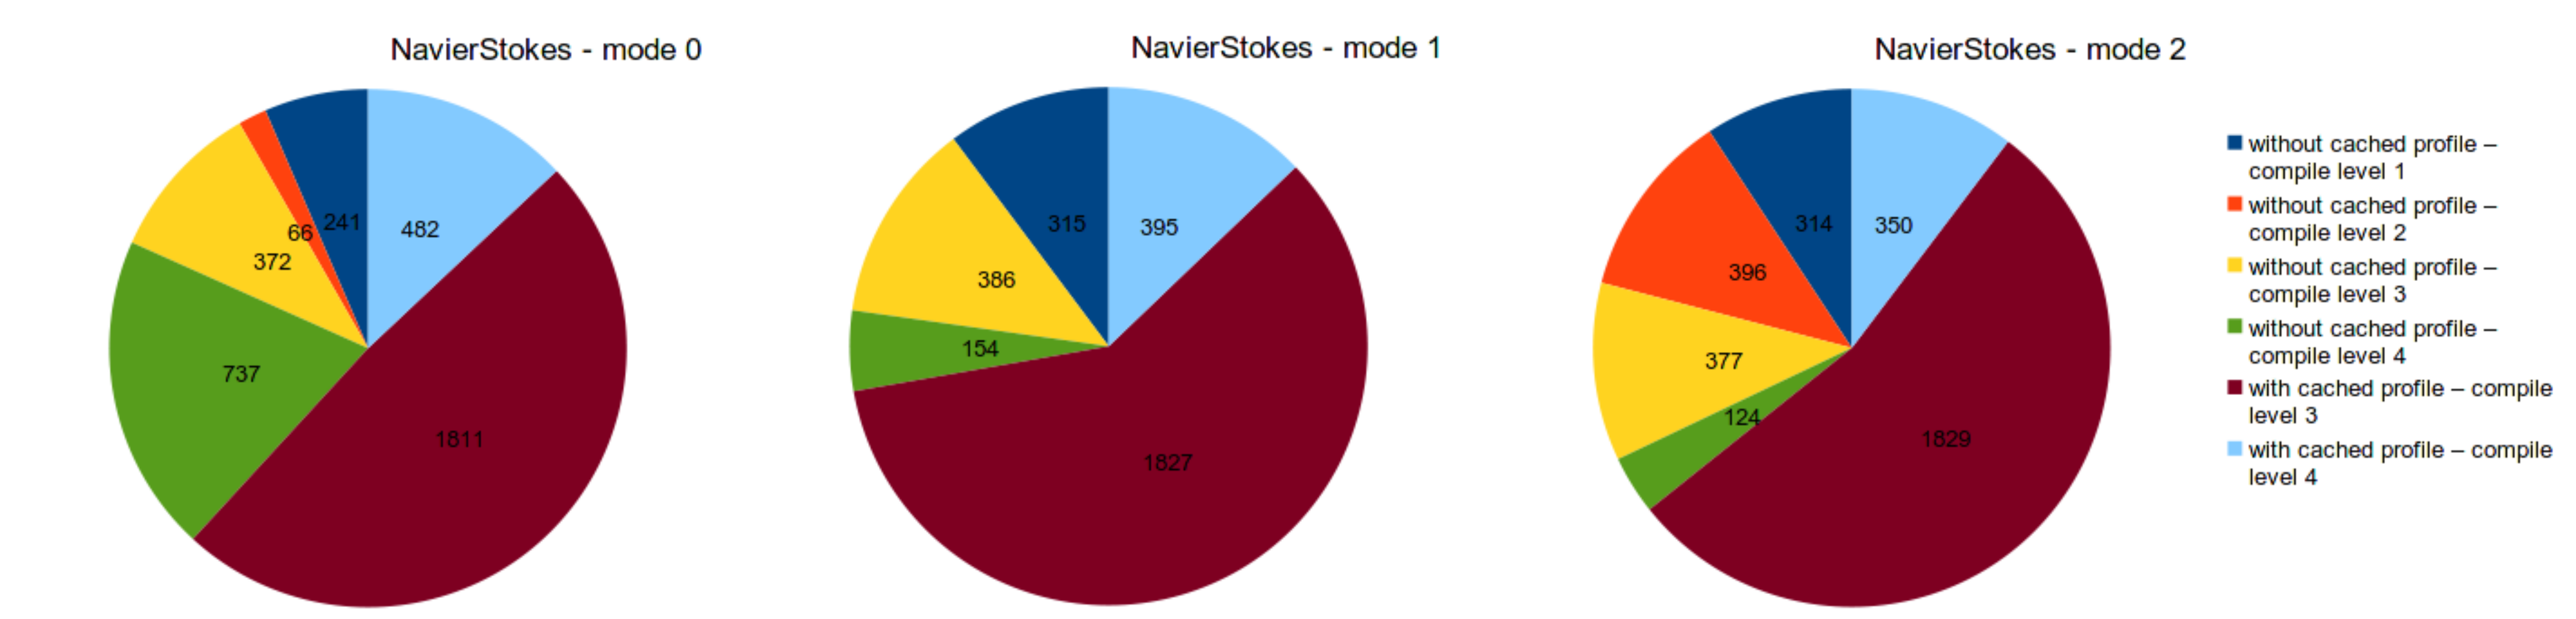
\includegraphics[width=1.0\textwidth]{figures/navierstokes_compilations.png}
    \caption{Ratio of compilations Octane NavierStokes benchmark}
    \label{f:navierstokes_compilations}
  \end{center}
\end{figure}
% --------------------------- Compilation cake compress ------------------
\begin{figure}[ht]
  \begin{center}
    \centering
    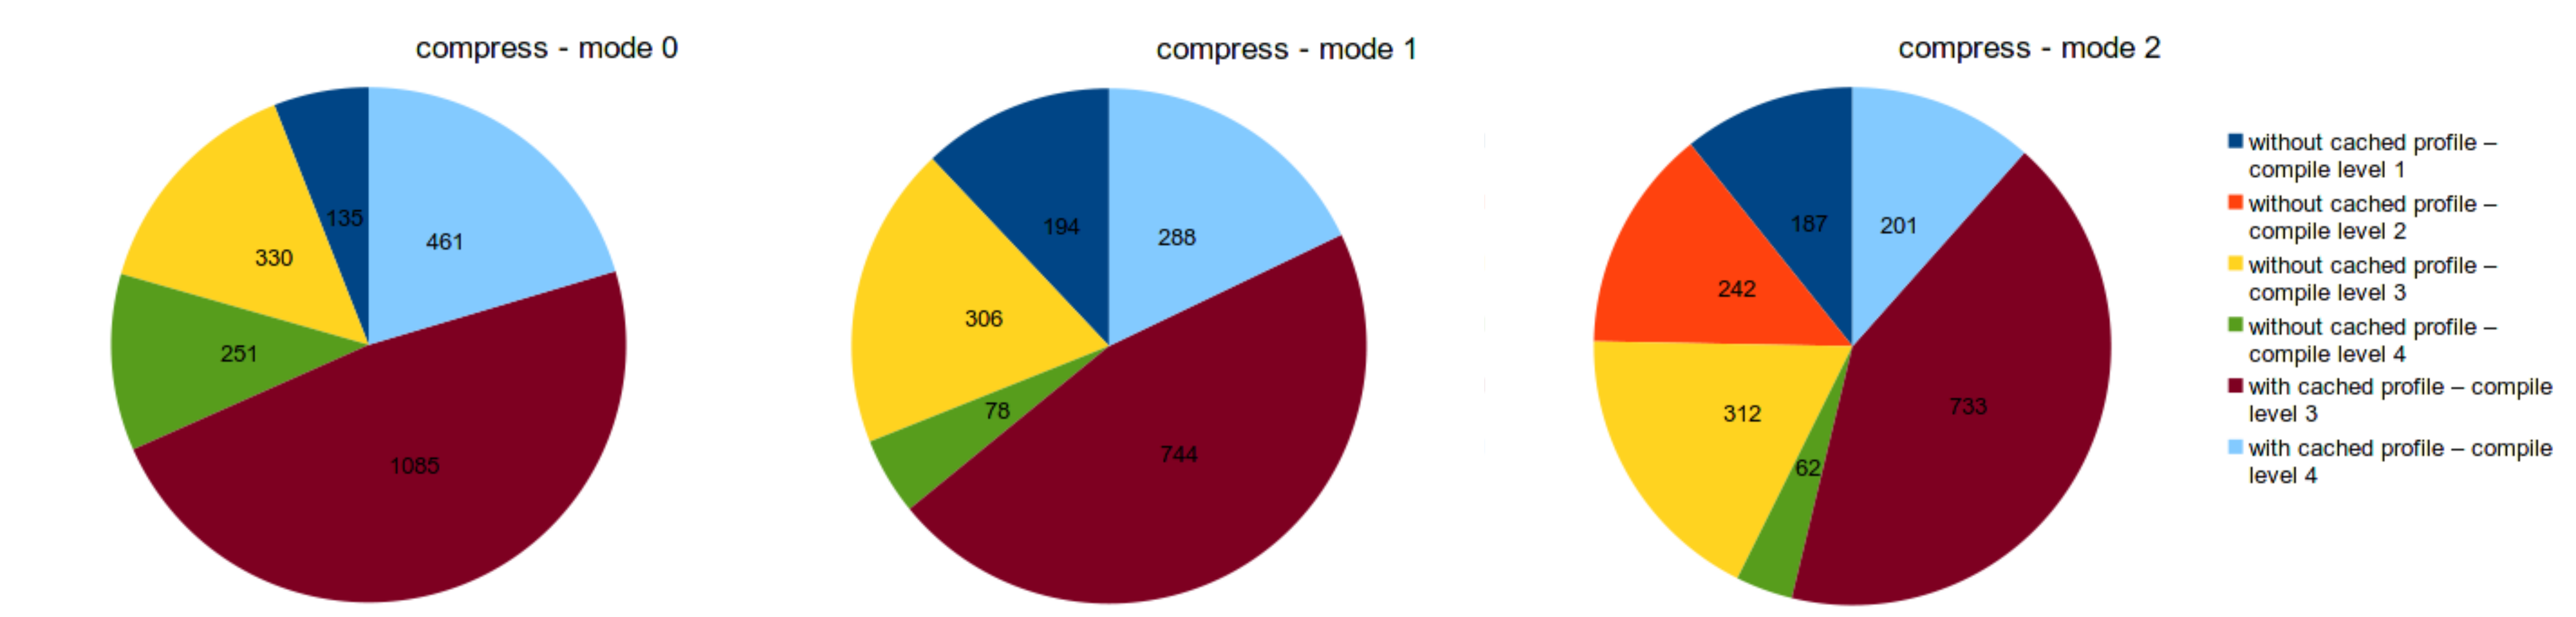
\includegraphics[width=1.0\textwidth]{figures/compress_compilations.png}
    \caption{Ratio of compilations SPECjvm compress benchmark}
    \label{f:compress_compilations}
  \end{center}
\end{figure}
% --------------------------- Compilation cake sparse.large ------------------
\begin{figure}[ht]
  \begin{center}
    \centering
    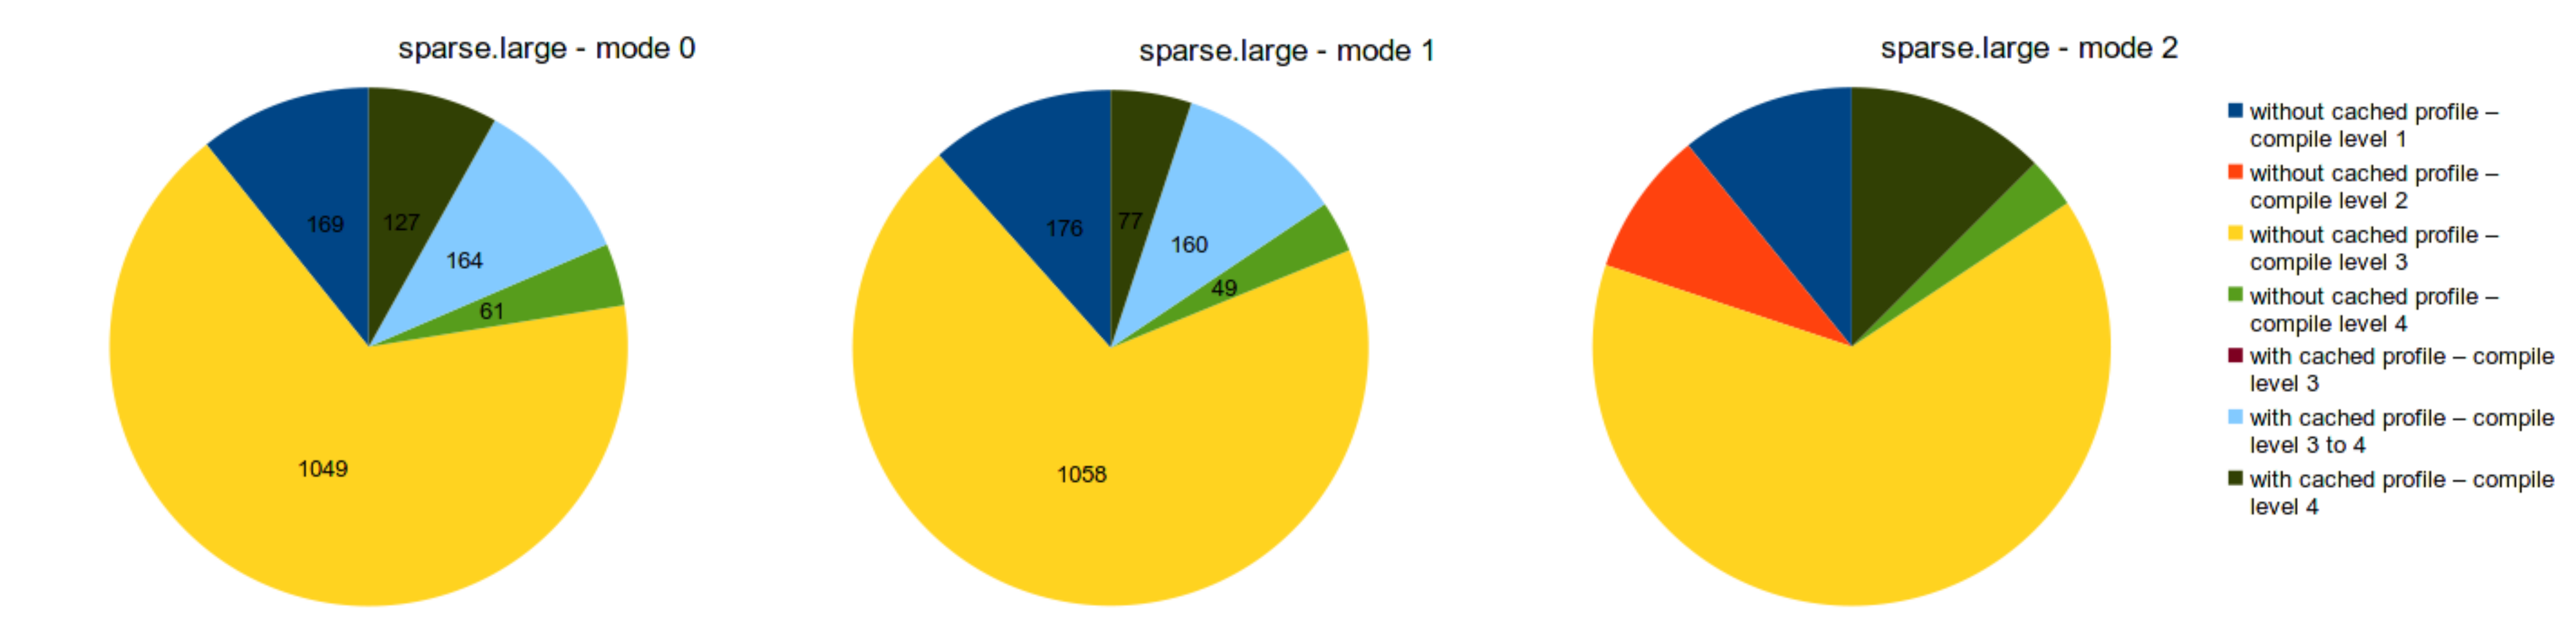
\includegraphics[width=1.0\textwidth]{figures/sparselarge_compilations.png}
    \caption{Ratio of compilations SPECjvm sparse.large benchmark}
    \label{f:sparselarge_compilations}
  \end{center}
\end{figure}
\clearpage
\section{Time spent in compiler}
\label{s:perf_compiletime}
Since our benchmark system has 16 cores and both the JVM itself and some of the benchmarks are multi-threaded, it is challenging to find the limiting factor for the JVM's performance. It is likely, that the CPU time spent compiling the methods with the JVM could not be used for the actual benchmark execution anyway since most of the benchmarks parallelism is limited.
This would mean, that a higher load on the compiler does not necessarily negatively affect performance.
\\\\
However, we are interested to know, whether using cached profiles also results in less time spent in HotSpot's compilers.
We use the built-in JVM flag \texttt{-XX:+CITime} which prints out detailed timing information about the C1 and C2 compiler.
We restrict our analysis to the total time spent in both compilers and take a look at all benchmarks again.
\\\\
Figure \ref{f:all_variation_compiletime_c1} shows the time spent in the C1 compiler for all SPECjvm benchmarks relative to the baseline. The results for all three modes are different. \texttt{Mode 0} increases the time in all benchmarks except mpegaudio. Even in benchmarks that achieve better performance in \texttt{Mode 0} than in the baseline (e.g. compress achieved a 30\% performance increase), the C1 compiler time is 50\% higher. The one exception, mpegaudio, had a performance loss of around 7\% when using cached profiles.
In contrast, \texttt{Mode 1} significantly reduces the time spent in the C1 compiler in all SPECjvm benchmarks. There is again no correlation between decrease of compile time and performance.
\texttt{Mode 2} has the lowest impact on the compile time, which in most cases is not significant.
\begin{figure}[ht!]
  \begin{center}
    \centering
    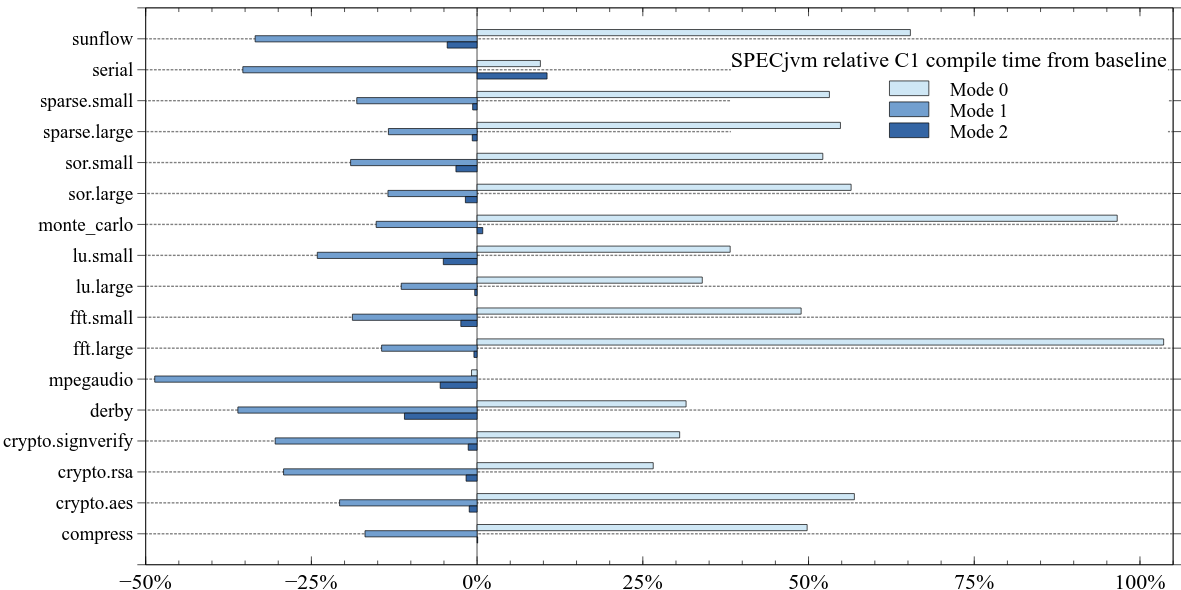
\includegraphics[width=1.0\textwidth]{figures/all_variation_compiletime_c1.png}
    \caption{Time spent in C1 compilations relative to baseline (SPECjvm)}
    \label{f:all_variation_compiletime_c1}
  \end{center}
\end{figure}
\\
The same statistics are drawn for the C2 compiler in Figure \ref{f:all_variation_compiletime_c2}. 
\texttt{Mode 0} shows similar behavior in C2 as in C1. It increases the time spent in the compiler by up to 160\% (in crypto.signverify).
The effect in \texttt{Mode 1} is not clear as the impact varies from -40\% in serial up to +52\% in crypto.signverify. \texttt{Mode 2} seems to decrease the time in C2 significantly. However, when looking back at Section \ref{s:perf_specjvm_warmup}, \texttt{Mode 2} did not perform better than the other two modes.
\begin{figure}[ht!]
  \begin{center}
    \centering
    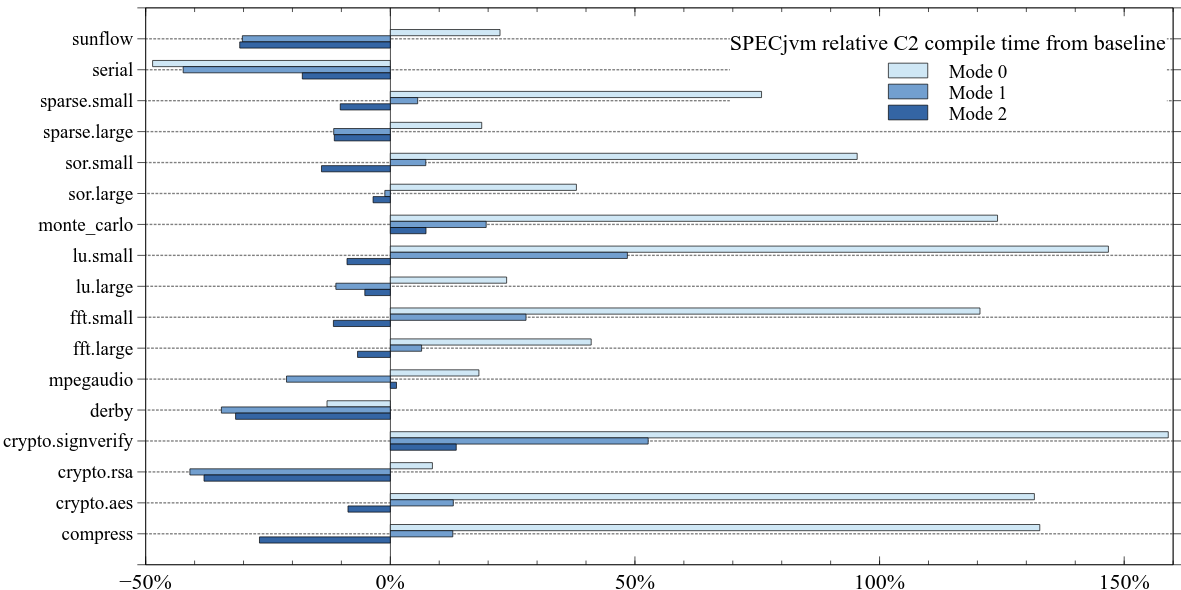
\includegraphics[width=1.0\textwidth]{figures/all_variation_compiletime_c2.png}
    \caption{Time spent in C2 compilations relative to baseline (SPECjvm)}
    \label{f:all_variation_compiletime_c2}
  \end{center}
\end{figure}
\\
We repeat the analysis for the Octane benchmarks and the results are drawn for C1 in Figure \ref{f:octane_variation_compiletime_c1} and C2 in Figure \ref{f:octane_variation_compiletime_c2}.\\
\begin{figure}[ht]
  \begin{center}
    \centering
    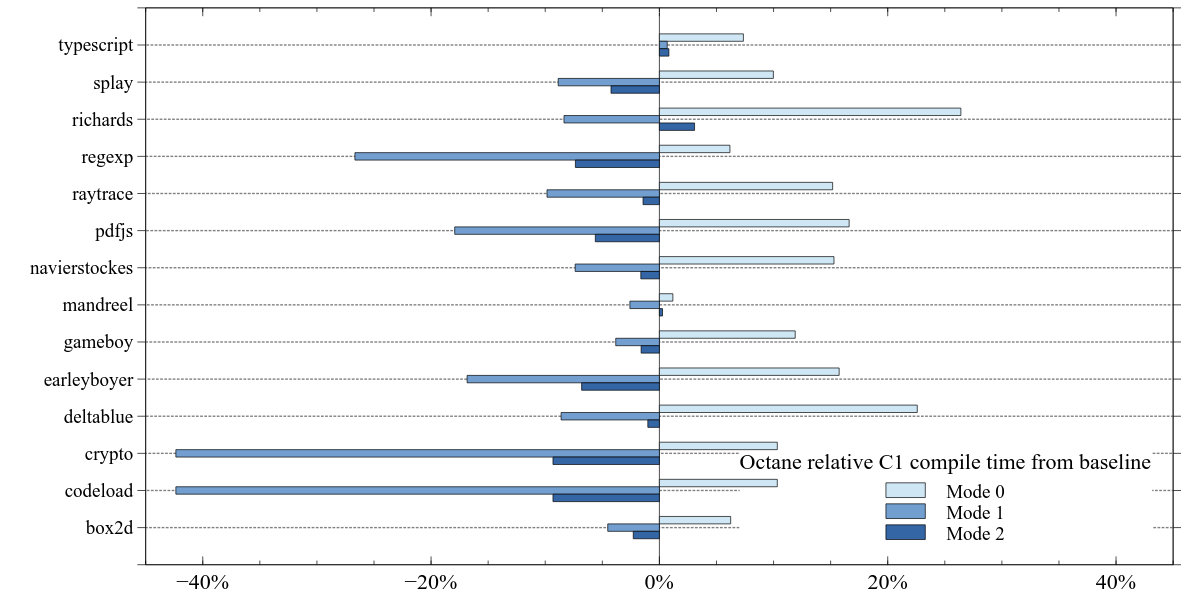
\includegraphics[width=1.0\textwidth]{figures/octane_variation_compiletime_c1.png}
    \caption{Time spent in C1 compilations relative to baseline (Octane)}
    \label{f:octane_variation_compiletime_c1}
  \end{center}
\end{figure}
\begin{figure}[ht]
  \begin{center}
    \centering
    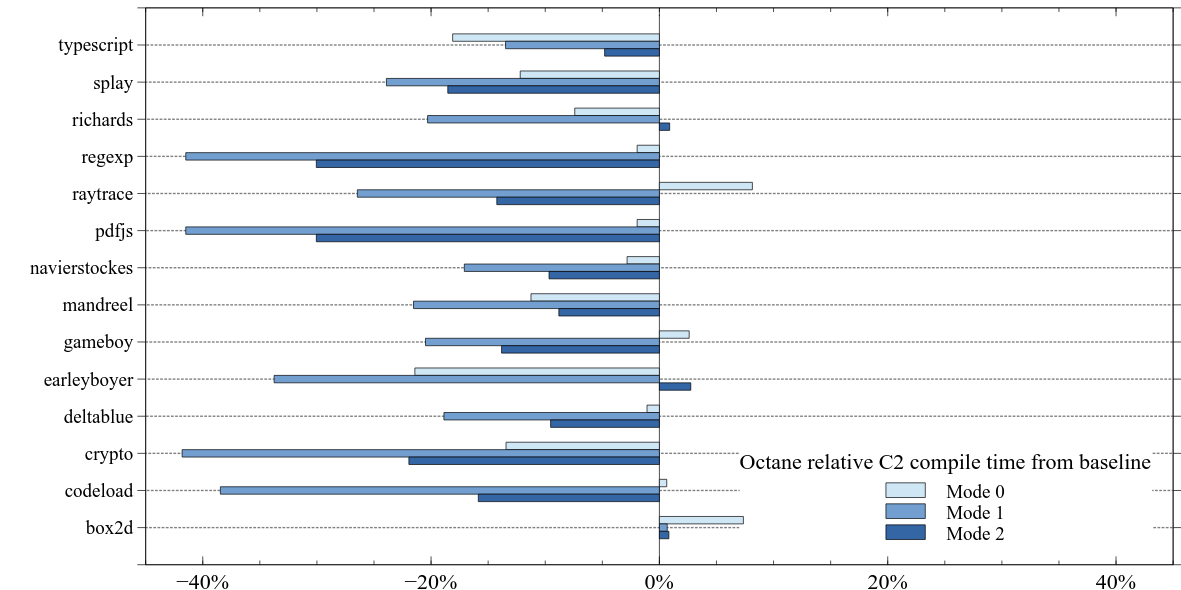
\includegraphics[width=1.0\textwidth]{figures/octane_variation_compiletime_c2.png}
    \caption{Time spent in C2 compilations relative to baseline (Octane)}
    \label{f:octane_variation_compiletime_c2}
  \end{center}
\end{figure}
For C1, \texttt{Mode 0} again increases the time spent in the compiler. However, the average increase of time is 10\%, while SPECjvm averages at a much higher percentage of 47\%.
\texttt{Mode 1} achieves the highest decrease and \texttt{Mode 2} has again less significant impact.
\\\\
In contrary to SPEVjvm, in Octane all modes decrease C2 compile time on average. There are a few expections, like Raytrace and Box2D, but in most benchmarks even \texttt{Mode 0} reduces the time spent in C2. Mode 1 has the most impact (-21\% on average), followed by Mode 2 (-10\% on average) and Mode 1 (-4\% on average).
\\\\
Since more time spent in the compiler could actually mean more compilations or longer compilations, let us recall the number of compilations discussed in Section \ref{s:perf_compilenumber}. For \texttt{Mode 0}, we experience a lower number of C1 compilations compared to the baseline in the Octane benchmarks and a higher number in SPECjvm. However, the actual time spent in C1 increase in both benchmark suites. We conclude that, especially in Octane, individual C1 compilations take longer, when cached profiles are involved. \texttt{Mode 1} invokes less C1 compilations in all benchmarks and the total time also decreased. Based on these benchmarks, we can not tell if per compilation time also decreased. In \texttt{Mode 2}, the number of C1 compilations does not change significantly compared to the baseline and the impact on the total compile time was also small.
\\\\
\texttt{Mode 0} puts more load on C2 than the baseline which can explain the increase of compile time for the SPECjvm benchmarks. On the other hand, the Octane ones spend less time in C2 and, together with more compilations, this means that the time per compilation decreases. The results for \texttt{Mode 1} are similar but the increase in number of compilations is less. In SPECjvm, the impact on compile time is also less (there are even benchmarks, where compile time decreases) but higher for the Octane benchmarks. The number of C2 compilations does not differ much when cached profiles in \texttt{Mode 2} are used. Nevertheless, in all benchmarks less time is spent in the C2 compiler.
\\\\
These results show, that using cached profiles can significantly decrease the time spent in compilation in \texttt{Mode 1} and \texttt{Mode 2}. In a system, where a program's performance is influenced by the time spent in JVM internal methods this could decrease the number of CPU time needed by the JVM and increase the resources available to the executed program. However, we can not determine a correlation between the change in compilation time and the benchmark performance in our setup.
\clearpage
\section{Effect of interpreter profiles}
\label{s:perf_interpreter_profiles}
Our system makes use of two types of cached profiles. Profiles, that are gathered by the interpreter and used by the C1 compiler and profiles that are gathered by a C1 compiled method and used when compiling with C2.
\\\\
We added a HotSpot flag that allows us to specify the minimum level of a compilation that dumps profiles (\texttt{-XX:DumpProfilesMinTier=}level).
Previous measurements were done setting this to level=3, which dumps profiles during Level 3 (C1 with full profiles) and Level 4 (C2 compilations.
\\\\
However, we are also interested how the system performance changes when only C2 compiler profiles are used. The system will then only use cached profiles where a C2 compilation took place in the previous profile generation run. We use the same setup as before and run the individual SPECjvm (see Figure \ref{f:others_warmup_wo_i}) and Octane (see Figure \ref{f:octane_wo_i}) benchmarks. 
\\\\
Most of the benchmarks do not show significantly different results compared to Section \ref{s:perf_benchmark}. There are a few benchmarks, where individual modes now improve the performance, while having a performance drop when both, C1 and C2 profiles, are used (e.g. NavierStokes \texttt{Mode 0}). But we also experience the other way around, for example in benchmark Splay \texttt{Mode 2}. In these individual cases, we believe, that for example a benchmarks C1 compilation does not profit from having cached profiles and therefore using them will even decrease performance (also see Section \ref{s:initializingprofiles}).
\\\\
The results let us conclude that the performance differences to the baseline are mostly due to the code quality of C2 compilations. Even though the number of C1 compilations is usually a lot higher than the number of C2 compilations, C2 compilations seem more critical to the methods performance.
\begin{figure}[ht]
  \begin{center}
    \centering
    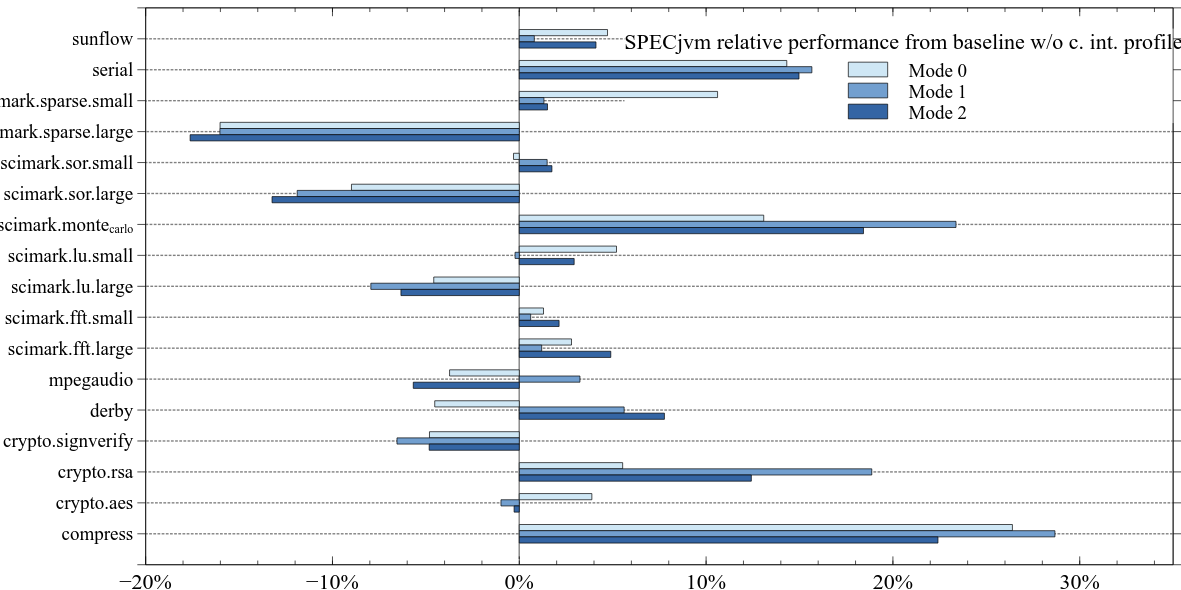
\includegraphics[width=1.0\textwidth]{figures/all_warmup_variation_wo_i.png}
    \caption{Warmup performance without using cached interpreter profiles relative to baseline (SPECjvm)}
    \label{f:others_warmup_wo_i}
  \end{center}
\end{figure}
\begin{figure}[ht]
  \begin{center}
    \centering
    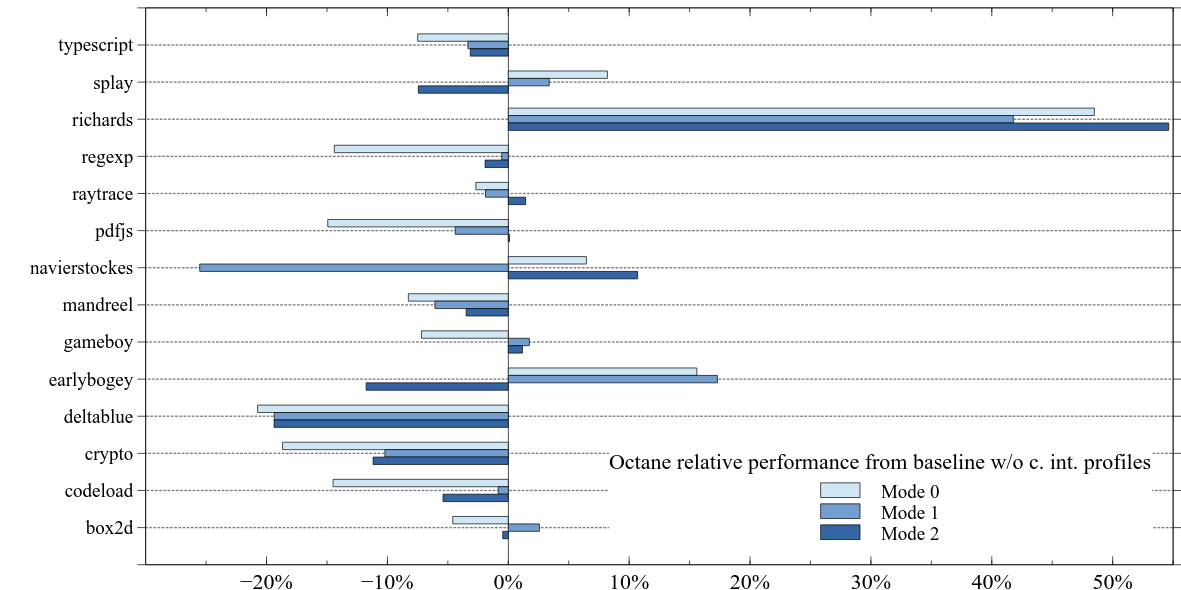
\includegraphics[width=1.0\textwidth]{figures/octane_variation_wo_i.png}
    \caption{Performance without using cached interpreter profiles relative to baseline (Octane)}
    \label{f:octane_wo_i}
  \end{center}
\end{figure}
\clearpage
\section{Effect of intrinsified methods}
\label{s:perf_intrinsics}
Most modern JVMs use \textit{method intrinsics} to further optimize commonly used Java core library methods \cite{intrinsics_talk}.
This means, that the JIT compiler does not compile the method based on the Java bytecode but instead replaces it with a predefined, and manually optimized assembly code snippet. The current list of methods where intrinsics are available can be found in the code reference \cite{code_intrinsics}.
\\\\
Intrinsics are mostly used in C1 and C2 compilations and the emitted code is independent of the current available profiling information.
This means, if many methods of a benchmark are intrinsified, the influence of profiles, and therefore cached profiles as well, decreases.
We want to know, whether this could be an issue in the benchmarks we looked at. A compilation of an intrinsified method has no advantage of having a rich profiling information but will still be influenced by modified compilation thresholds. For example, lowering the threshold will intrinsify methods earlier and therefore speed up execution.
\\\\
The results of both benchmark suites with disabled method instrinsics can be found in Figures \ref{f:all_warmup_noi_variation} and Figure \ref{f:octane_noi_variation}.
For SPECjvm, we see that there are small performance differences in individual benchmarks but we can not conclude a major influence to the behavior of cached profiles and their influence on performance. Note, that the serial benchmark does not work with disabled intrinsics.
\\\\
Most of the Octane benchmarks do not work when intrinsics are disabled and the ones that work run a lot slower. We think in these benchmarks other unconsidered side effects occur and an analysis regarding cached profiles would not be accurate.
\begin{figure}[ht]
  \begin{center}
    \centering
    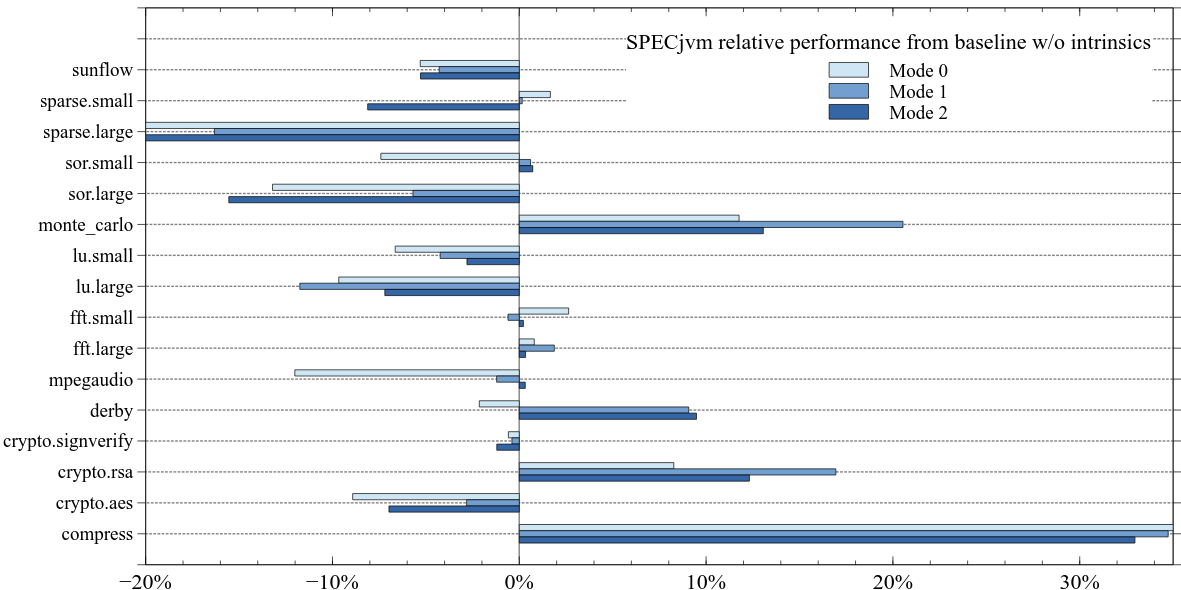
\includegraphics[width=1.0\textwidth]{figures/all_warmup_noi_variation.png}
    \caption{Warmup performance without intrinsified methods relative to baseline (SPECjvm)}
    \label{f:all_warmup_noi_variation}
  \end{center}
\end{figure}
\begin{figure}[ht]
  \begin{center}
    \centering
    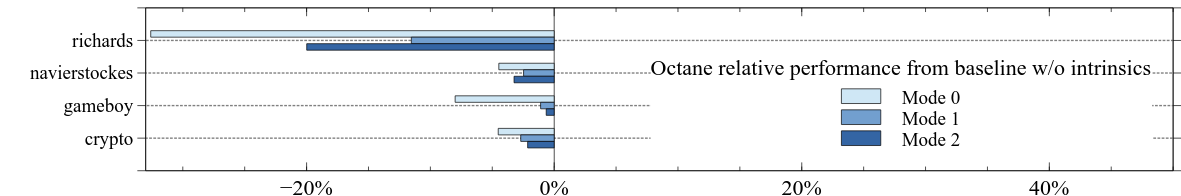
\includegraphics[width=1.0\textwidth]{figures/octane_noi_variation.png}
    \caption{Performance without intrinsified methods relative to baseline (Octane)}
    \label{f:octane_noi_variation}
  \end{center}
\end{figure}
